\documentclass[
    12pt,
    oneside,
    a4paper,
    brazil
]{abntex2}

\usepackage{lmodern}
\usepackage[T1]{fontenc}
\usepackage[utf8]{inputenc}
\usepackage{amsmath}
\usepackage{amssymb}
\usepackage{booktabs}
\usepackage{array}
\usepackage{xcolor}
\usepackage{pgfgantt}
\usepackage{adjustbox}
\usepackage{soul}
\usepackage{graphicx}


\begin{document}

    \pretextual
    % ---
% Impressão da Capa
% ---
  \begin{capa}%
    \begin{figure}[h!]%
        \centering%
        
\includegraphics[scale=1.2]{figs/logo.png}%
      \end{figure}%
    \center
	\ABNTEXchapterfont\large{Universidade Federal do ABC \\ Centro de Matemática, Computação e Cognição \\ Projeto de Graduação em Computação}
	%\vspace{1.5cm}

    \vfill
    \ABNTEXchapterfont\bfseries\LARGE{Otimização do plano de voo de VANTs para coleta de dados de sensores IoT}
    \vfill

	%\vfill
	\ABNTEXchapterfont\large{Lucas de Medeiros Santos}
	\vfill
%	
    \large{Santo André}, \large{agosto de 2025}

    \vspace*{1cm}
  \end{capa}
% ---

    \begin{resumo}
        A coleta de dados em redes de sensores IoT por meio de veículos aéreos não tripulados (UAVs) exige o planejamento cuidadoso da trajetória de voo, de modo a equilibrar a qualidade da informação coletada e o consumo energético do veículo. Este trabalho propõe uma formulação de Programação Linear Inteira Mista (PLIM) para o problema de otimização do plano de voo de um UAV dedicado à coleta de dados de sensores distribuídos em uma área geográfica. O modelo discretiza o horizonte da missão em intervalos de tempo (\textit{slots}) e representa a movimentação do veículo sobre um grafo completo de nós (sensores e base), incorporando um modelo de potência de asa rotativa para estimar o custo energético de cada deslocamento e dos períodos de pairar (\textit{hovering}). A \textit{Age of Information} (AoI) é utilizada como medida da relevância temporal dos dados, e a missão é otimizada de forma multiobjetivo lexicográfica: maximiza-se primeiro a AoI efetivamente coletada e, em seguida, minimiza-se a energia consumida. A formulação foi implementada no resolvedor Gurobi e avaliada em 36 cenários, variando a quantidade de sensores e o tamanho do mapa, com parâmetros físicos do DJI Matrice 300 RTK e do Parrot Anafi USA, e comparada a heurísticas construtivas de referência (\textit{Nearest Neighbor}, AoI-Greedy e Score-Greedy). Os resultados indicam que o modelo exato encontra soluções de boa qualidade nas escalas avaliadas e que a restrição de visita única a cada sensor constitui uma escolha eficiente, obtendo qualidade de AoI equivalente à de uma variante com revisitas, porém com consumo energético significativamente menor.

        \vspace{\onelineskip}
        \noindent\textbf{Palavras-chave}: UAV; Internet das Coisas; \textit{Age of Information}; otimização; programação linear inteira mista; eficiência energética.
    \end{resumo}

    \textual

    \section{Introdução}

A coleta eficiente de dados em redes de sensores sem fio (WSNs, do inglês \textit{wireless sensor networks}) é um componente essencial para a operação de sistemas de monitoramento ambiental, infraestrutura inteligente e aplicações em Internet das Coisas (IoT). Nessas redes, dispositivos de baixo consumo energético são distribuídos em uma área de monitoramento para coletar grandezas físicas (temperatura, umidade, vibração, entre outras) e transmiti-las periodicamente a um ponto central de coleta. Em cenários nos quais a conectividade com infraestrutura fixa é limitada ou inexistente, veículos aéreos não tripulados (UAVs, do inglês \textit{unmanned aerial vehicles}) têm sido explorados como coletores móveis, oferecendo flexibilidade de deslocamento, escalabilidade e maior cobertura espacial \cite{liu2018uavWSN}.

A utilização de UAVs como \emph{sinks} móveis — coletores de dados que absorvem as informações transmitidas pelos sensores da rede — introduz desafios complexos de planejamento de voo, coordenação e gerenciamento energético. O desempenho da coleta está diretamente relacionado a fatores como tempo de voo, energia disponível, capacidade de comunicação ar–terra e a estratégia de sobrevoo adotada. Três estratégias principais são identificadas na literatura \cite{messaoudi2023survey}: \textit{hovering} (o UAV paira estático sobre o sensor durante a coleta), \textit{fly-by} (o drone sobrevoa em movimento contínuo, coletando dados em trânsito) e híbrida (combinação das duas anteriores). A avaliação desse tipo de distema envolve, além de métricas clássicas (throughput agregado, latência, capacidade por nó e consumo energético), a \emph{Age of Information} (AoI), que mede o tempo desde a última atualização recebida de um sensor até o presente momento, crucial quando dados desatualizados perdem rapidamente relevância~\cite{messaoudi2023survey}.

A literatura recente propõe modelagens e técnicas para planejamento de trajetórias, incluindo (i) partição de área em células para coleta periódica \cite{liu2018uavWSN}, (ii) esquemas de coleta baseados em aprendizado por reforço profundo \cite{zhang2018drlrvc} e (iii) estratégias cooperativas entre múltiplos UAVs visando aumentar capacidade e eficiência energética \cite{yang2020surveyUAVIoT}. Em particular, o uso coordenado de múltiplos UAVs, quando bem modelado, pode proporcionar ganhos expressivos em capacidade por nó e no tempo de vida da rede em relação a abordagens com UAV único \cite{liu2018uavWSN,yang2020surveyUAVIoT}. Embora esses resultados motivem abordagens multiagente, este trabalho concentra-se no cenário com um único UAV, de modo a isolar o impacto das decisões de trajetória e consumo energético sobre as métricas de qualidade da coleta e viabilizar uma formulação de otimização exata tratável.

Neste trabalho, propomos uma formulação geral do problema de planejamento de voo para UAVs atuando como coletores de dados em WSNs, com foco em aspectos energéticos e operacionais. A modelagem visa abranger diferentes parâmetros envolvidos na coleta, como altura de voo, número de sensores, cobertura por célula e capacidade de coleta por unidade de tempo. O objetivo é otimizar simultaneamente métricas de eficiência energética, cobertura, tempo de coleta e AoI, oferecendo uma base para análise de desempenho e desenvolvimento de algoritmos de otimização aplicáveis a diferentes cenários de IoT assistida por UAVs.

O restante deste documento está organizado da seguinte forma. A Seção~2 apresenta os trabalhos relacionados e um comparativo com a proposta deste trabalho. A Seção~3 aborda a fundamentação teórica, incluindo conceitos de WSN, AoI, UAVs e modelos de energia e comunicação. A Seção~4 define os objetivos do trabalho. A Seção~5 descreve a modelagem matemática do problema de otimização. A Seção~6 detalha a metodologia experimental e os resultados obtidos para os dois modelos de drone avaliados. Por fim, a Seção~7 apresenta o cronograma de atividades.


    \chapter{Trabalhos Relacionados}
\label{sec:relacionados}

Diversos trabalhos na literatura abordaram a utilização de veículos aéreos não tripulados (VANTs) como ferramentas para coleta de dados em redes de sensores da Internet das Coisas (IoT), com foco em otimização de trajetória, eficiência energética e minimização da idade da informação (AoI).

Wei et al.~\cite{wei2022survey} apresentam um extenso levantamento sobre coleta de dados assistida por VANTs em IoT, abordando os principais desafios e tecnologias associadas, como clustering de sensores, modos de coleta (voo pairado, sobrevoo e híbrido) e planejamento de trajetória conjunto com alocação de recursos. Os autores destacaram que a flexibilidade dos VANTs permite melhorar significativamente a cobertura e eficiência da coleta de dados em ambientes complexos. Além disso, o trabalho propõe uma taxonomia das abordagens existentes e discute algoritmos baseados em teoria dos grafos, teoria da otimização e inteligência artificial para resolver o problema.

Messaoudi et al.~\cite{messaoudi2023survey} também forneceram uma revisão abrangente dos esquemas de coleta de dados baseados em VANTs, com foco em desafios como consumo energético, atraso na coleta, limitação de mobilidade e segurança. O artigo propôs uma categorização das aplicações e técnicas, discutindo ainda abordagens energéticas como redes com carregamento sem fio e estratégias para minimizar a AoI. Os autores enfatizaram a importância de integrar VANTs de forma inteligente para garantir eficiência e longevidade da rede IoT, além de sugerirem direções futuras promissoras, como o uso de VANTs energizados por comunicação e integração com redes 5G/6G.

Liu et al.~\cite{liu2018uavWSN} investigaram o desempenho da coleta de dados em redes de sensores sem fio (WSNs) com apoio de VANTs, especialmente em cenários sem infraestrutura de comunicação. O artigo propôs um modelo onde a região de cobertura é dividida em células e diferentes estratégias de trajeto são projetadas para um ou múltiplos VANTs. Os autores derivaram a capacidade por nó (\textit{per-node capacity}), que depende do número de células, da altura dos VANTs, da densidade de sensores e da capacidade energética das aeronaves. Concluiu-se que o uso de múltiplos VANTs aumenta significativamente essa capacidade em comparação com apenas um VANT. Além disso, o artigo determina o número ótimo de células para maximizar o desempenho da rede e valida os resultados teóricos com simulações. O trabalho contribui para o entendimento do impacto de diferentes parâmetros na eficiência da coleta de dados, oferecendo orientações práticas para o planejamento de missões VANT em WSNs.

Zhang et al.~\cite{zhang2018drlrvc} propuseram uma estrutura baseada em aprendizado profundo para otimizar a coleta de dados por veículos autônomos em cidades inteligentes, com foco especial em eficiência energética. O trabalho introduziu o framework \textit{DRL-RVC}, que utiliza redes neurais convolucionais para extrair características relevantes (como distribuição de amostras e fluxo de tráfego), e redes Q profundas para controlar VANTs e veículos autônomos de recarga. Os VANTs realizam a coleta de dados priorizando áreas de maior relevância, enquanto veículos autônomos terrestres são mobilizados para oferecer recarga, contornando restrições urbanas. Os resultados de simulação mostraram alta efetividade e robustez da abordagem proposta.

Yang et al.~\cite{yang2020surveyUAVIoT} realizam uma análise abrangente das principais questões na coleta de dados assistida por VANTs em ambientes de IoT, abordando desde o impacto do posicionamento dos nós sensores até o planejamento de trajetória e navegação autônoma. O estudo destacou que uma implantação eficiente dos sensores, aliada à otimização de parâmetros de voo (como velocidade e altitude) e a técnicas de compressão, clustering e classificação de dados, é fundamental para maximizar a eficiência energética e a quantidade de dados coletados. Os autores também enfatizaram o papel de algoritmos de planejamento de rota e desvio inteligente de obstáculos, sugerindo que abordagens inspiradas em aprendizado por reforço podem melhorar significativamente o desempenho de VANTs na coleta em larga escala, especialmente em terrenos complexos e de difícil acesso.

A Tabela~\ref{tab:comparativo} sintetiza a comparação entre os trabalhos revisados e a proposta deste trabalho. As duas últimas colunas indicam se cada trabalho trata a energia e a AoI como \emph{objetivos de otimização}, ou seja, grandezas efetivamente minimizadas ou maximizadas por um modelo, e não apenas como temas discutidos de forma qualitativa. Sob esse critério, os \textit{surveys} de Wei et al., Messaoudi et al. e Yang et al. mapeiam desafios de consumo energético e de atualidade dos dados, mas não formulam um modelo que os otimize. O trabalho analítico de Liu et al. concentra-se em maximizar a capacidade por nó, sem tratar energia nem AoI como objetivo. Zhang et al. otimizam a eficiência energética por aprendizado profundo, porém não consideram a AoI. Constata-se, assim, que nenhum trabalho anterior otimiza AoI e energia conjuntamente.

Este trabalho preenche essa lacuna ao formular o problema de coleta de dados como um programa linear inteiro misto (MILP) com dois objetivos conflitantes: maximizar a AoI coletada pelos sensores e minimizar o consumo energético do VANT. A abordagem lexicográfica empregada garante soluções ótimas exatas, ao passo que o uso de parâmetros físicos reais de dois modelos de drone (DJI Matrice 300 RTK e Parrot Anafi USA) confere aderência prática ao modelo. Diferentemente dos trabalhos que consideram múltiplos VANTs, optou-se pelo cenário com VANT único, o que permite isolar o impacto das decisões de trajetória e energia sobre a qualidade da coleta de forma controlada.

\begin{table}[htbp]
  \centering
  \caption{Comparativo entre trabalhos relacionados e a proposta deste trabalho. As colunas ``Otimiza energia'' e ``Otimiza AoI'' indicam se o trabalho adota cada grandeza como objetivo de otimização, e não apenas como tema de discussão.}
  \label{tab:comparativo}
  \small
  \adjustbox{max width=\linewidth}{%
  \begin{tabular}{>{\raggedright\arraybackslash}p{4.3cm}
                  >{\centering\arraybackslash}p{1.1cm}
                  >{\centering\arraybackslash}p{1.7cm}
                  >{\raggedright\arraybackslash}p{2.6cm}
                  >{\centering\arraybackslash}p{1.7cm}
                  >{\centering\arraybackslash}p{1.4cm}}
    \toprule
    \textbf{Trabalho} & \textbf{Ano} & \textbf{N° VANTs} & \textbf{Método} & \textbf{Otimiza energia} & \textbf{Otimiza AoI} \\
    \midrule
    Wei et al.~\cite{wei2022survey} & 2022 & Múltiplos & Revisão & Não & Não \\
    Messaoudi et al.~\cite{messaoudi2023survey} & 2023 & Múltiplos & Revisão & Não & Não \\
    Liu et al.~\cite{liu2018uavWSN} & 2018 & Múltiplos & Analítico & Não & Não \\
    Zhang et al.~\cite{zhang2018drlrvc} & 2018 & Múltiplos & Aprendizado profundo & Sim & Não \\
    Yang et al.~\cite{yang2020surveyUAVIoT} & 2020 & Múltiplos & Revisão & Não & Não \\
    \midrule
    \textbf{Este trabalho} & \textbf{2026} & \textbf{Único} & \textbf{MILP (exato)} & \textbf{Sim} & \textbf{Sim} \\
    \bottomrule
  \end{tabular}}
\end{table}


    \section{Fundamentação Teórica}
\label{sec:fundamentacao}

\subsection{Programação Linear e Otimização Inteira}
\label{sec:prog-linear}

A otimização matemática trata da escolha, dentre um conjunto de alternativas viáveis, daquela que minimiza (ou maximiza) uma medida de desempenho. Quando tanto a função objetivo quanto as restrições que delimitam as alternativas são expressas por relações lineares, o problema é dito de \emph{programação linear}. Esta seção introduz os conceitos de programação linear, sua extensão ao domínio inteiro e o caso misto, que constitui a base formal do modelo proposto neste trabalho.

\paragraph{Programação Linear (PL).}
Um problema de programação linear busca otimizar uma função objetivo linear sujeita a um conjunto de restrições também lineares. Na forma padrão, pode ser escrito como
\begin{align}
    \min_{x}\quad & c^{\top} x \notag \\
    \text{sujeito a}\quad & A x \le b, \label{eq:pl-padrao} \\
    & x \ge 0, \notag
\end{align}
onde $x \in \mathbb{R}^n$ é o vetor de variáveis de decisão (contínuas), $c \in \mathbb{R}^n$ define os coeficientes da função objetivo, e $A \in \mathbb{R}^{m \times n}$ e $b \in \mathbb{R}^m$ descrevem as restrições. O conjunto de pontos que satisfazem todas as restrições é a \emph{região factível}, que forma um poliedro convexo. Um resultado central da otimização linear estabelece que, se o problema admite solução ótima, então existe um \emph{vértice} (ponto extremo) da região factível que é ótimo \cite[Propriedade~2.2]{arenales2007pesquisa}; de modo equivalente, basta procurar o ótimo entre as soluções básicas factíveis, que correspondem aos vértices da região. Essa propriedade fundamenta o método \emph{simplex}, que percorre vértices adjacentes da região factível, melhorando a função objetivo a cada passo até alcançar o ótimo \cite{arenales2007pesquisa}.

\paragraph{Programação Linear Inteira (PLI).}
Em muitas aplicações práticas, as variáveis de decisão representam grandezas indivisíveis ou escolhas lógicas e, portanto, devem assumir apenas valores inteiros. Acrescentar a exigência $x \in \mathbb{Z}^n$ ao problema~\eqref{eq:pl-padrao} caracteriza a \emph{programação linear inteira}. Um caso particularmente importante é o das variáveis \emph{binárias} ($x \in \{0,1\}^n$), capazes de modelar decisões do tipo sim/não, como ``visitar ou não um nó'' ou ``ativar ou não uma rota''. Diferentemente da PL, a PLI é, em geral, computacionalmente muito mais difícil de resolver: a restrição de integralidade torna o conjunto factível discreto (não convexo) e o número de combinações inteiras a examinar cresce rapidamente com a quantidade de variáveis, tornando inviável a enumeração completa das soluções em instâncias de grande porte \cite{arenales2007pesquisa}.

\paragraph{Programação Linear Inteira Mista (MILP).}
Quando apenas parte das variáveis é restrita a valores inteiros, enquanto as demais permanecem contínuas, tem-se um problema de \emph{programação linear inteira mista} (MILP, do inglês \textit{Mixed-Integer Linear Programming}) \cite{arenales2007pesquisa}. Essa formulação é especialmente expressiva para problemas de roteamento e escalonamento, nos quais variáveis binárias capturam decisões discretas (por exemplo, qual aresta percorrer) e variáveis contínuas representam grandezas físicas acumuladas (por exemplo, energia ou tempo).

\paragraph{Resolução por \textit{branch-and-bound}.}
A principal técnica para resolver problemas de PLI e MILP de forma exata é o \emph{branch-and-bound} \cite{land1960branchbound, arenales2007pesquisa}. A ideia central é dividir o problema em subproblemas menores (\emph{branching}) e usar limitantes para descartar (\emph{bounding}) aqueles que comprovadamente não podem conter a solução ótima, evitando testar todas as combinações possíveis. Esse método, em conjunto com técnicas de planos de corte, está implementado em resolvedores de otimização como o Gurobi, adotado neste trabalho.

\paragraph{Relação com este trabalho.}
O problema de planejamento de voo abordado neste trabalho é formulado como um MILP: variáveis binárias descrevem a posição do UAV, os deslocamentos e as coletas, enquanto variáveis contínuas registram a energia acumulada e a \emph{Age of Information} dos sensores. Termos não lineares, como o produto entre a AoI e a decisão de coleta, são convertidos em restrições lineares por meio de técnicas de linearização (Seção~\ref{sec:modelagem}, Equações~\eqref{eq:lin-a}--\eqref{eq:lin-c}), preservando a estrutura linear necessária à resolução exata pelo Gurobi.

\subsection{IoT e WSN}

A Internet das Coisas (IoT, do inglês \textit{Internet of Things}) é um paradigma que integra objetos físicos (sensores, atuadores e dispositivos embarcados) à infraestrutura digital por meio de protocolos de comunicação sem fio, permitindo a coleta, transmissão e processamento autônomo de dados do ambiente \cite{yang2020surveyUAVIoT}. Dentro desse paradigma, as redes de sensores sem fio (WSNs, do inglês \textit{Wireless Sensor Networks}) constituem uma das tecnologias de suporte mais consolidadas: consistem em conjuntos de nós de baixo consumo energético, distribuídos em uma área de interesse, responsáveis por amostrar grandezas físicas (temperatura, umidade, vibração, entre outras) e encaminhá-las periodicamente a um ponto de coleta centralizado \cite{liu2018uavWSN}.

Em aplicações de monitoramento ambiental, agricultura de precisão, vigilância urbana e resposta a desastres, os nós sensores frequentemente operam em áreas de difícil acesso ou sem cobertura de infraestrutura fixa. Nesse contexto, UAVs têm sido explorados como \emph{sinks} móveis, percorrendo a área de missão para coletar dados diretamente dos sensores \cite{wei2022survey,messaoudi2023survey}.

\subsection{Age of Information (AoI)}

Uma métrica central para avaliar a qualidade da informação coletada nessas redes é a \emph{Age of Information} (AoI), introduzida para quantificar a \emph{frescor} dos dados disponíveis em um ponto de destino \cite{messaoudi2023survey}. Intuitivamente, a AoI mede há quanto tempo a última atualização de um determinado sensor foi recebida. Quanto maior a AoI, mais desatualizada é a informação disponível.

\paragraph{Definição formal.}

No modelo de tempo discreto adotado neste trabalho, o horizonte de missão é dividido em \emph{slots} de duração $\Delta t$. Para cada sensor $j \in S$, define-se $A_{j,t}$ como a \textbf{idade da informação} do sensor $j$ no início do slot $t$, medida em número de slots desde a última coleta. Sua dinâmica é dada por:

\begin{align}
    A_{j,1} &= A_j^0, \qquad \forall j \in S, \tag{AoI-0} \\[4pt]
    A_{j,t+1} &=
    \begin{cases}
        0, & \text{se } v_{j,t} = 1 \text{ (coleta realizada no slot } t\text{)}, \\[4pt]
        A_{j,t} + 1, & \text{se } v_{j,t} = 0 \text{ (sem coleta)},
    \end{cases}
    \tag{AoI-1}
\end{align}

onde $A_j^0$ é o valor inicial carregado do estado persistido entre missões e $v_{j,t} \in \{0,1\}$ é a variável de decisão que indica se o sensor $j$ é coletado no slot $t$.

Quando o UAV coleta o sensor $j$ no slot $t$, a AoI é zerada no slot seguinte, pois o destino passa a dispor de uma atualização recente. Caso contrário, a AoI cresce em uma unidade por slot, refletindo o envelhecimento da informação. Maximizar a soma $\sum_{j,t} A_{j,t}\, v_{j,t}$, isto é, priorizar sensores com AoI mais alta no momento da coleta, é equivalente a maximizar o \emph{ganho informacional} acumulado pela missão, incentivando visitas a nós cujos dados estejam mais desatualizados.

\subsection{UAVs}

Veículos aéreos não tripulados (UAVs, do inglês \textit{Unmanned Aerial Vehicles}), popularmente chamados de drones, são aeronaves controladas remotamente ou de forma autônoma, sem piloto a bordo \cite{messaoudi2023survey}. Originalmente desenvolvidos para fins militares, os UAVs passaram a ser amplamente utilizados em aplicações civis como mapeamento, agricultura de precisão, vigilância, entrega de cargas e, em particular, coleta de dados em redes IoT \cite{wei2022survey}.

Do ponto de vista da propulsão, os UAVs mais relevantes para coleta de dados em WSNs se dividem em dois grandes grupos:

\begin{itemize}
    \item \textbf{Asa fixa (\textit{fixed-wing})}: aeronaves que geram sustentação pelo perfil aerodinâmico das asas durante o deslocamento horizontal. Possuem maior autonomia e velocidade de cruzeiro, mas não conseguem pairar estáticos sobre um ponto e exigem velocidade mínima de voo para manter sustentação.
    \item \textbf{Asa rotativa (\textit{rotary-wing})}: aeronaves com um ou mais rotores horizontais (helicópteros, quadricópteros, hexacópteros). Têm menor autonomia e velocidade máxima, mas são capazes de realizar \emph{hover} (permanecer estacionários no ar), o que facilita a comunicação direta com sensores fixos no solo \cite{zeng2019rotarywing}.
\end{itemize}

Neste trabalho, adota-se o modelo de asa rotativa, coerente com os UAVs utilizados nos experimentos (DJI Matrice 300 RTK e Parrot Anafi USA).

\subsubsection{Modos de coleta}
\label{sec:modos-coleta}

A estratégia de sobrevoo adotada pelo UAV determina como e quando a comunicação com os sensores ocorre. Três modos principais são identificados na literatura \cite{messaoudi2023survey,wei2022survey}:

\begin{itemize}
    \item \textbf{\textit{Hovering}}: o UAV desloca-se até a posição do sensor e paira estático acima dele pelo tempo necessário para completar a transmissão. Garante máxima qualidade de enlace (menor distância e velocidade relativa nula), à custa de maior consumo energético para manter o voo estacionário.
    \item \textbf{\textit{Fly-by}}: o drone sobrevoa o sensor em movimento contínuo, realizando a coleta em trânsito. Reduz o tempo total de missão e o consumo associado ao hover, porém a janela de comunicação é curta e a qualidade do enlace pode ser comprometida pela variação da distância e pelo efeito Doppler.
    \item \textbf{Híbrido}: combina os dois modos anteriores, selecionando a estratégia mais adequada para cada sensor conforme seus requisitos de enlace e localização.
\end{itemize}

No modelo adotado neste trabalho, a coleta ocorre exclusivamente em modo \textit{hovering}: o UAV deve permanecer parado sobre o sensor durante um slot inteiro para que a transmissão seja considerada bem-sucedida. Esse pressuposto é modelado pela restrição $v_{j,t} = x_{jjt}$, que vincula a coleta ao \emph{self-loop} do grafo de movimento (ver Seção~\ref{sec:modelagem}).

\subsubsection{Restrições operacionais}

A operação de um UAV de asa rotativa é condicionada por dois limites principais:

\begin{itemize}
    \item \textbf{Capacidade de bateria ($E^{\max}$)}: a energia armazenada na bateria limita o tempo total de missão. O consumo depende da velocidade de deslocamento e do tempo em hover, conforme o modelo de potência de Zeng et al.~\cite{zeng2019rotarywing} descrito na Seção~\ref{sec:modelagem}.
    \item \textbf{Horizonte temporal ($T_f$)}: o número máximo de slots disponíveis para a missão, que define o comprimento do plano de voo a ser otimizado.
\end{itemize}

A interação entre esses dois limites é central para o problema de otimização formulado neste trabalho: aumentar o número de sensores visitados exige mais deslocamentos e mais tempo em hover, elevando o consumo e eventualmente inviabilizando a missão dentro do orçamento energético disponível.

\subsection{Modelo de energia de UAV de asa rotativa}

O consumo energético de UAVs de asa rotativa é fortemente dependente do regime de voo: manter-se estacionário (\emph{hover}) exige potência elevada para sustentar o peso do veículo contra a gravidade, enquanto o deslocamento horizontal apresenta um ponto ótimo de eficiência situado entre o custo de sustentação e o arrasto aerodinâmico.

Para modelar esse comportamento com fidelidade física, este trabalho adota o modelo de potência proposto por Zeng et al.~\cite{zeng2019rotarywing}, que decompõe a potência instantânea de um rotor em três componentes:

\begin{enumerate}
    \item \textbf{Potência de perfil das pás}: cobre o arrasto viscoso das pás ao girarem. Em translação horizontal, as pás avançam e recuam assimetricamente contra o fluxo de ar, fazendo esta parcela crescer proporcionalmente ao quadrado da velocidade.
    \item \textbf{Potência induzida}: energia transferida ao ar para gerar sustentação (empuxo). Domina em \emph{hover}, decresce até um mínimo com o aumento da velocidade e volta a crescer em velocidades elevadas.
    \item \textbf{Potência de arrasto parasita}: captura o arrasto aerodinâmico da fuselagem e de componentes expostos ao fluxo; cresce proporcionalmente ao cubo da velocidade e é dominante apenas em altas velocidades.
\end{enumerate}

A expressão matemática da potência $P(V)$ em função da velocidade horizontal $V$ é apresentada na Seção~\ref{sec:modelagem} (Equação~\eqref{eq:potencia}). Em \emph{hover} ($V = 0$), o modelo simplifica-se para $P_{\mathrm{hov}} = P_0 + P_i$, onde $P_0$ é a potência de perfil e $P_i$ é a potência induzida, ambas avaliadas em velocidade nula. Com os parâmetros do DJI Matrice 300 RTK ($P_0 = 79{,}86$\,W, $P_i = 88{,}63$\,W), obtém-se $P_{\mathrm{hov}} \approx 168{,}5$\,W.

Os parâmetros físicos completos utilizados nos experimentos, obtidos de \cite{zeng2019rotarywing}, são: $P_0 = 79{,}86$\,W, $P_i = 88{,}63$\,W, $U_{\mathrm{tip}} = 120$\,m/s (velocidade da ponta da pá), $v_0 = 4{,}03$\,m/s (velocidade induzida em \emph{hover}), $\rho = 1{,}225$\,kg/m³ (densidade do ar) e $C_{DS} = 0{,}01509$\,m² (coeficiente de arrasto parasita efetivo, dado por $c_d \cdot s \cdot A$, com $c_d = 0{,}6$, $s = 0{,}05$ e $A = 0{,}503$\,m²). Esses parâmetros são adotados nos dois conjuntos de experimentos; a diferença entre os UAVs está na capacidade de bateria $E^{\max}$: $2$\,MJ para o DJI Matrice 300 RTK e $141{,}372$\,kJ para o Parrot Anafi USA (capacidade nominal real do equipamento).

O custo energético de cada transição no grafo de movimento é obtido multiplicando a potência calculada pela duração do slot $\Delta t = 10$\,s (Equação~\eqref{eq:custo-energia}, Seção~\ref{sec:modelagem}). As restrições de acumulação e capacidade de energia no modelo MILP são apresentadas na Seção~\ref{sec:modelagem} (Equações~\eqref{eq:energia-inicial}--\eqref{eq:energia-capacidade}).

\subsection{Modelo de comunicação}

Em sistemas UAV-IoT, modelos de comunicação detalhados descrevem explicitamente o canal de rádio (perda de percurso, desvanecimento, relação sinal-ruído e protocolos de controle de acesso ao meio) condicionando a taxa de sucesso à qualidade do enlace~\cite{wei2022survey,messaoudi2023survey}. Esses modelos são relevantes quando a mobilidade do UAV provoca variações significativas de distância ou ângulo durante a coleta.

Neste trabalho, adota-se um modelo de comunicação binário simplificado, coerente com o modo de coleta \emph{hovering} descrito na Seção~\ref{sec:modos-coleta}. O pressuposto central é que a transmissão de dados ocorre com sucesso garantido se, e somente se, o UAV permanecer estacionário diretamente acima do sensor durante um slot completo de duração $\Delta t$.

Não são modelados aspectos de camada de enlace como taxa de dados, modulação, interferência entre sensores ou protocolo MAC. A coleta é representada pela variável binária $v_{j,t} \in \{0,1\}$, vinculada ao \emph{self-loop} de permanência do UAV sobre o nó sensor (Equação~\eqref{eq:coleta}, Seção~\ref{sec:modelagem}).

Esta simplificação é adequada por três motivos:

\begin{enumerate}
    \item \textbf{Distância mínima:} ao pairar sobre o sensor, o UAV minimiza a distância de enlace, garantindo SNR suficiente para tecnologias de curto alcance como IEEE 802.15.4, Zigbee ou LoRa.
    \item \textbf{Canal estacionário:} em \emph{hover}, a velocidade relativa entre drone e sensor é nula, eliminando o efeito Doppler e reduzindo as flutuações de desvanecimento.
    \item \textbf{Foco em roteamento:} o objetivo da formulação é otimizar a trajetória e o escalonamento de visitas; o desempenho do enlace de rádio, condicionalmente à presença de \emph{hover}, é tratado como garantido. Modelos de canal mais detalhados podem ser incorporados em extensões futuras.
\end{enumerate}

 
    \section{Objetivos}

O objetivo principal deste trabalho é avaliar o problema de otimização de plano de voo de veículos aéreos não tripulados (UAVs) com foco na coleta de dados de sensores IoT distribuídos em uma área geográfica a partir de uma abordagem matemática.

\subsection*{Objetivos específicos}

\begin{itemize}
    \item Formular o problema utilizando tempo discretizado e variáveis de decisão apropriadas.
    \item Modelar múltiplos objetivos, como a  a eficiência energética (dados coletados por unidade de energia), idade da informação (AoI) dos sensores, e tempo total de voo do UAV.
%    \begin{itemize}
%        \item Maximização da eficiência energética (dados coletados por unidade de energia).
%        \item Minimização da idade da informação (AoI) dos sensores.
%        \item Minimização do tempo total de voo do UAV.
%    \end{itemize}
%    \item Incorporar restrições operacionais relevantes, como:
%    \begin{itemize}
%        \item Limites de energia disponíveis.
%        \item Restrições de comunicação (raio de alcance dos sensores).
%        \item Restrições de deslocamento baseadas em velocidade máxima.
%    \end{itemize}
%    \item Comparar diferentes abordagens para formulação multiobjetivo, incluindo soma ponderada e método $\varepsilon$-restrito.
    \item Implementar a formulação em um resolvedor de otimização (como Gurobi) e realizar experimentos computacionais, comparando resultados ao que já existe na literatura.
\end{itemize}

    
    \chapter{Modelagem Matemática do Problema de Otimização de Plano de Voo para UAVs}
    \label{sec:modelagem}

    \section{Descrição do Problema}
    
    O problema de otimização de plano de voo para UAVs consiste em determinar a trajetória ótima que um drone deve seguir para coletar dados de um conjunto de sensores IoT distribuídos em uma área geográfica. O objetivo principal é maximizar a quantidade de dados coletados enquanto se minimiza o consumo de energia do drone e a idade da informação (Age of Information, AoI), respeitando suas limitações operacionais. O drone parte de uma posição inicial conhecida, deve visitar um subconjunto de sensores dentro do seu alcance de comunicação, e se dirigir a uma posição final (que pode ser igual à inicial). Durante o voo, o drone consome energia de acordo com sua velocidade e manobras, e coleta dados quando está dentro do raio de comunicação dos sensores. A qualidade da comunicação entre o drone e os sensores depende da distância entre eles. Este problema pode ser modelado como um problema de otimização combinatória com restrições de energia, tempo de voo, e requisitos de comunicação, considerando também a idade dos dados nos sensores para priorizar a coleta de informações mais antigas.
    
    Esta formulação é relevante para aplicações como monitoramento ambiental, agricultura de precisão, vigilância urbana e resposta a desastres, onde a coleta eficiente e oportuna de dados de sensores distribuídos é crucial para a tomada de decisões.

O modelo de comunicação adotado é simplificado: assume-se que a transmissão ocorre com sucesso sempre que o UAV permanece pairando (\textit{hovering}) diretamente sobre o sensor durante um slot completo de duração $\Delta t$. Não são modelados aspectos de camada de enlace como modulação, interferência ou protocolo MAC; a coleta é representada por uma variável binária que indica se o drone está posicionado sobre o sensor no instante correspondente (ver Equação~\eqref{eq:coleta}).


    \section{Parâmetros e Variáveis}

O modelo representa o voo do UAV como uma sequência de estados discretos no tempo, divididos em slots de duração $\Delta t$. O espaço de movimentação é modelado como um grafo completo sobre o conjunto de nós $N = S \cup \{b\}$ (sensores e base), com coordenadas bidimensionais $(x, y)$. O custo energético de cada transição é determinado pelo modelo de potência de asa rotativa em função da velocidade de voo. As variáveis de decisão binárias controlam a posição e os deslocamentos do UAV ao longo do horizonte temporal; variáveis contínuas registram a energia acumulada e a \textit{Age of Information} (AoI) de cada sensor a cada slot. A solução ótima define uma sequência de posições do UAV que maximiza a informação coletada respeitando a restrição de capacidade de bateria $E^{\max}$. As Tabelas~\ref{tab:parametros} e~\ref{tab:variaveis} listam, respectivamente, os parâmetros e as variáveis de decisão do modelo.

    \begin{table}[htbp]
      \centering
      \caption{Parâmetros do Modelo}
      \label{tab:parametros}
      \begin{tabular}{>{\raggedright\arraybackslash}p{2.2cm} >{\raggedright\arraybackslash}p{10cm}}
        \toprule
        \textbf{Notação} & \textbf{Descrição} \\
        \midrule
        \multicolumn{2}{l}{\textit{Conjuntos}} \\
        \midrule
        $T$ & Conjunto de intervalos de tempo discretos: $T = \{1, 2, \ldots, T_f\}$ \\
        $S$ & Conjunto de sensores distribuídos na área: $S = \{1, 2, \ldots, n\}$ \\
        $b$ & Índice da base (nó inicial e final do voo) \\
        $N$ & Conjunto de locais onde o drone pode permanecer parado (sensores $S$ e base $b$): $N = S \cup \{b\}$ \\
        $A = N \times N$ & Conjunto de arestas dirigidas (inclui \textit{self-loop} $(i,i)$) \\
        \midrule
        \multicolumn{2}{l}{\textit{Parâmetros Geométricos}} \\
        \midrule
        $S_j$ & Posição fixa do sensor $j \in S$: $S_j = (x_j, y_j, h_j)$ \\
        $d_{ij}$ & Distância euclidiana entre os locais $i,j \in N$ \\
        \midrule
        \multicolumn{2}{l}{\textit{Parâmetros de Tempo e Energia}} \\
        \midrule
        $\Delta t$ & Duração de cada intervalo de tempo (slot) \\
        $E^{\max}$ & Capacidade máxima de energia da bateria do UAV \\
        $A_j^0$ & Idade inicial da informação do sensor $j \in S$ antes do voo \\
        $M_A$ & Constante \textit{Big-M} segura para AoI (por exemplo, $M_A \ge \max_j A_j^0 + T_f$) \\
        \midrule
        \multicolumn{2}{l}{\textit{Parâmetros do Modelo de Potência do UAV}} \\
        \midrule
        $P_0$ & Termo de potência de perfil das pás do rotor \\
        $\Pi$ & Termo de potência induzida em voo \\
        $U_{\text{tip}}$ & Velocidade da ponta da hélice \\
        $v_0$ & Velocidade induzida em \textit{hover} \\
        $\rho$ & Densidade do ar \\
        $C_{DS}$ & Parâmetro de arrasto parasita efetivo (área equivalente) \\
        $c_{ij}$ & Custo energético associado à aresta $(i,j)$ em um slot \\
        \bottomrule
      \end{tabular}
    \end{table}
    
    \begin{table}[htbp]
      \centering
      \caption{Variáveis de Decisão}
      \label{tab:variaveis}
      \begin{tabular}{>{\raggedright\arraybackslash}p{2.2cm} >{\raggedright\arraybackslash}p{10cm}}
        \toprule
        \textbf{Notação} & \textbf{Descrição} \\
        \midrule
        $p_{n,t}$ & Indica se o drone está no local $n \in N$ no início do slot $t \in T$ \\
        $x_{ijt}$ & Indica se o drone realiza o movimento de $i \to j$ entre os slots $t$ e $t+1$ \\
        $v_{j,t}$ & Indica se o drone realiza coleta de dados do sensor $j \in S$ no slot $t$ \\
        $y_j$ & Indica se o sensor $j$ foi visitado (coletado) ao menos uma vez ao longo do horizonte \\
        $E_t$ & Energia acumulada pelo drone até o início do slot $t \in T$ \\
        $A_{j,t}$ & Idade da informação do sensor $j$ no início do slot $t$ \\
        $w_{j,t}$ & Variável auxiliar que representa $A_{j,t}\cdot v_{j,t}$ (AoI efetivamente coletada) \\
        \bottomrule
      \end{tabular}
    \end{table}

    
    \section{Formulação do Problema}
    
    Seja $T = \{1, 2, \dots, \tau\}$ o conjunto de intervalos de tempo discretos. O objetivo
    é planejar a trajetória de um ou mais UAVs para coleta eficiente de dados em sensores IoT, respeitando restrições de mobilidade, energia, e requisitos de comunicação. O problema pode ser formulado pelas equações nas subseções a seguir.

    \subsection{Definição do Grafo de Movimento}

    O conjunto de posições possíveis para o UAV é dado por    
    $N = S \cup \{b\}$, onde $b$ representa a base.  
    Diferentemente de modelos que usam grafos esparsos, aqui adotamos $A = N \times N$, um grafo dirigido completo com \emph{self-loops}.  
    Isso significa que:
    
    \begin{itemize}
        \item o UAV pode transitar de qualquer nó para qualquer outro em um único slot (pressuposto do grafo completo; na prática, transições longas são desincentivadas pelo custo energético $c_{ij}$);
        \item o caso $(i,i)$ modela \textbf{hover}, isto é, o UAV permanece parado;
        \item a dinâmica de movimento é totalmente determinada pelas variáveis $x_{ijt}$. 
    \end{itemize}
    
    O uso de um grafo completo fornece maior generalidade, permitindo representar tanto deslocamentos quanto posicionamento estático.

    \paragraph{Interpretação de $x_{ijt}$.}

    A variável binária $x_{ijt}$ indica que o UAV se encontra no nó $i$ no início do slot $t$ e estará no nó $j$ no início do slot $t+1$.
    Assim:

    \[
    x_{ijt} =
    \begin{cases}
    1, & \text{se o UAV realiza a transição } i \to j, \\[4pt]
    0, & \text{caso contrário}.
    \end{cases}
    \]

    O caso especial
    \[
    x_{iit} = 1
    \]
    implica que o UAV permanece parado (\emph{hover}), o que também é utilizado para caracterizar coletas via $v_{j,t} = x_{jjt}$.

    \subsection{Modelo de Energia e Potência do UAV}

    O modelo de consumo energético utilizado é baseado no modelo de potência para VANTs de asa rotativa descrito por \cite{zeng2019rotarywing}, que considera três componentes:

    \begin{itemize}
        \item potência de perfil das pás;
        \item potência induzida;
        \item potência de arrasto parasita.
    \end{itemize}

    A potência consumida pelo UAV quando se desloca com velocidade $V$ é dada por:

    \begin{align}
    P(V) &=
    P_0\!\left(1 + 3\frac{V^2}{U_{\text{tip}}^2}\right)
    \;+\;
    \Pi \sqrt{
            \sqrt{1 + \frac{V^4}{4 v_0^4}}
            \;-\;
            \frac{V^2}{2 v_0^2}
        }
    \;+\;
    \frac{1}{2}\rho C_{DS} V^3 ,
    \label{eq:potencia}
    \end{align}

    onde $P_0$, $\Pi$, $U_\text{tip}$, $v_0$, $\rho$ e $C_{DS}$ são parâmetros físicos do UAV.

    Para uma transição $(i,j)$ em um slot de duração $\Delta t$, adotamos velocidade constante:

    \[
    V_{ij} = \frac{d_{ij}}{\Delta t}.
    \]

    Assim, o custo energético associado a uma aresta é:

    \begin{align}
        c_{ij} = P(V_{ij}) \, \Delta t.
        \label{eq:custo-energia}
    \end{align}

    A velocidade $V_{ij} = d_{ij}/\Delta t$ corresponde à hipótese de que cada transição entre dois nós é concluída em um único \textit{slot} de duração $\Delta t = 10$\,s a velocidade constante. Essa simplificação mantém o modelo de energia linear por aresta, mas implica que, em mapas grandes, as velocidades nominais podem superar a faixa operacional dos veículos: por exemplo, uma transição correspondente à diagonal de um mapa de $1000\times1000$\,m ($\approx 1414$\,m) exigiria $V_{ij} \approx 141$\,m/s, valor acima da velocidade da ponta da hélice $U_{\text{tip}} = 120$\,m/s e da velocidade de cruzeiro real do DJI Matrice 300 RTK e do Parrot Anafi USA. Trata-se de uma limitação da discretização em uma única transição por \textit{slot}: para os cenários de maior escala, os valores de energia devem ser interpretados como uma aproximação conservadora do custo de deslocamento, e não como reflexo de um perfil de voo fisicamente realizável a essa velocidade.

    O caso especial de \emph{hover} corresponde à aresta $(i,i)$, onde $V_{ii}=0$ e portanto:

    \[
    c_{ii} = P(0)\,\Delta t.
    \]

    Este modelo substitui formulações lineares simplificadas como $c_{ij} = k\, d_{ij}$, oferecendo maior precisão física na simulação do voo.


    \subsection{Funções Objetivo}

    A formulação do problema busca equilibrar dois aspectos fundamentais da missão: 
    (i) a maximização da quantidade de informação relevante coletada pelo UAV, medida pela Age of Information (AoI), e 
    (ii) a minimização do consumo total de energia durante o voo.  
    Esses objetivos, embora distintos, podem ser combinados em uma única função objetivo multicritério, refletindo o compromisso natural entre qualidade da coleta e economia energética.
    
    \paragraph{Maximização da Informação Coletada (AoI).}
    
    Para cada sensor $j$ e instante $t$, a variável $w_{j,t}$ representa a AoI efetivamente coletada naquele slot. Esse valor corresponde à idade da informação disponível no sensor no início do slot ($A_{j,t}$), desde que ocorra coleta ($v_{j,t}=1$), e é igual a zero caso contrário.
    
    Assim, a soma total de informação coletada ao longo da missão é dada por:
    
    \begin{align}
        f_{\text{AoI}}
        =
        \sum_{j \in S}
        \sum_{t = 1}^{T_f - 1}
        w_{j,t}.
        \label{eq:f-aoi}
    \end{align}
    
    Essa função incentiva visitas a sensores cujos dados estejam mais desatualizados, priorizando trajetórias que maximizem o impacto informacional da missão.
    
    \paragraph{Minimização do Consumo Energético.}
    
    A energia acumulada até o final do voo é representada pela variável $E_{T_f}$, que sintetiza todo o gasto resultante dos deslocamentos e períodos de \emph{hover}. Assim, o custo energético total da missão é expresso por:
    
    \begin{align}
        f_{\text{energia}}
        =
        E_{T_f}.
        \label{eq:f-energia}
    \end{align}
    
    Minimizar esse valor corresponde a promover trajetórias mais econômicas, aumentando a autonomia do veículo e preservando os recursos energéticos disponíveis.
    
    \paragraph{Função Objetivo Multicritério.}

    As duas componentes anteriores são combinadas por meio de uma otimização multiobjetivo \emph{lexicográfica} (hierárquica), e não de uma soma ponderada. Em vez de fixar um parâmetro de ponderação entre AoI e energia, atribui-se uma prioridade a cada objetivo: a maximização da AoI coletada recebe prioridade superior e a minimização da energia, prioridade inferior. Formalmente, resolve-se primeiro

    \begin{align}
        f_{\text{AoI}}^{\star}
        \;=\;
        \max\
        \sum_{j \in S}
        \sum_{t = 1}^{T_f - 1}
            w_{j,t},
        \label{eq:objetivo-aoi}
    \end{align}

    e, em seguida, entre todas as soluções que atingem $f_{\text{AoI}}^{\star}$, minimiza-se o consumo energético:

    \begin{align}
        \min\ E_{T_f}
        \qquad \text{sujeito a} \qquad
        \sum_{j \in S}\sum_{t=1}^{T_f-1} w_{j,t} = f_{\text{AoI}}^{\star}.
        \label{eq:objetivo-energia}
    \end{align}

    Dessa forma, o modelo primeiro garante a máxima informação coletada e, apenas como critério de desempate, escolhe entre as soluções ótimas aquela de menor gasto energético. Essa estrutura captura a essência do problema sem exigir a calibração de um peso relativo entre as grandezas: obter a maior quantidade de informação relevante possível e, dentre as alternativas igualmente boas nesse aspecto, a mais econômica em energia. Na implementação, essa hierarquia é definida diretamente pelo resolvedor (Gurobi) por meio de objetivos com prioridades distintas.

    \subsection{Restrições de Movimento}

    \begin{align}
      &\text{(i) início/fim na base:}& p_{b,1}&=1,\quad p_{b,T_f}=1 \label{eq:mov-base}\\
      &\text{(ii) unicidade de posição:}& \sum_{n\in N} p_{n,t} &= 1,\ \forall t\in\{1,\ldots,T_f\} \label{eq:mov-unicidade}\\
      &\text{(iii) fluxo por slot:}& \sum_{j\in N} x_{i j t} &= p_{i,t},\ \sum_{i\in N} x_{i j t} = p_{j,t+1},\ \forall t\in\{1,\ldots,T_f-1\} \label{eq:mov-fluxo}
    \end{align}

    As Restrições~\eqref{eq:mov-base}--\eqref{eq:mov-fluxo} modelam a dinâmica de movimento do UAV ao longo dos slots de tempo. A restrição~\eqref{eq:mov-base} fixa a base $b$ como ponto de partida e de chegada da missão, garantindo que o drone inicie o voo na base e retorne a ela no final do horizonte $T_f$. A restrição~\eqref{eq:mov-unicidade} impõe que, em cada slot $t$, o UAV esteja exatamente em um único nó $n \in N$, isto é, o drone não pode estar em dois locais ao mesmo tempo nem ``desaparecer'' do grafo. Já a restrição~\eqref{eq:mov-fluxo} garante a consistência do fluxo entre nós sucessivos: para cada slot $t$, o número de arestas saindo de um nó $i$ é igual à indicação de que o drone está em $i$ no início do slot, e o número de arestas chegando em um nó $j$ é igual à indicação de que o drone estará em $j$ no início do slot seguinte. Em conjunto, essas restrições asseguram que a trajetória do UAV é uma caminhada viável no grafo $N$ ao longo do horizonte de tempo.

    
    \subsection{Restrições de Comunicação}

    No modelo, uma coleta de dados ocorre somente quando o UAV permanece pairando sobre o sensor durante todo o slot.  
    
    Esse comportamento é modelado por meio de um \emph{self-loop} na aresta $(j,j)$:
    
    \begin{align}
        v_{j,t} = x_{j j t},
        \qquad \forall j \in S,\ t = 1,\ldots,T_f - 1.
        \label{eq:coleta}
    \end{align}
    
    Assim, $v_{j,t}=1$ indica que o drone está parado sobre o sensor $j$ durante o slot $t$ e realiza coleta.  
    Se o UAV estiver se deslocando entre quaisquer nós distintos $(i \ne j)$, então $x_{j j t} = 0$ e, portanto, nenhuma coleta ocorre.
    
    Também impomos que cada sensor seja visitado no máximo uma vez, conforme a restrição~\eqref{eq:visita-unica}:

    \begin{align}
        y_j &= \sum_{t=1}^{T_f - 1} v_{j,t},
        \label{eq:y-visita}\\[4pt]
        \sum_{t=1}^{T_f - 1} v_{j,t} &\le 1,
        \qquad \forall j \in S.
        \label{eq:visita-unica}
    \end{align}
    
    A variável $y_j$ indica se o sensor $j$ foi ou não visitado em algum instante.
    
    \subsection{Restrições de Energia}
    
    A energia acumulada no início do voo é nula:
    
    \begin{align}
        E_1 = 0. \label{eq:energia-inicial}
    \end{align}
    
    A evolução da energia é dada pela soma dos custos das arestas percorridas:
    
    \begin{align}
        E_{t+1}
        =
        E_t
        +
        \sum_{i \in N}
        \sum_{j \in N}
            c_{ij}\, x_{ijt},
        \qquad t = 1,\ldots,T_f - 1.
        \label{eq:energia-evolucao}
    \end{align}
    
    O consumo final acumulado não deve exceder a capacidade da bateria:
    
    \begin{align}
        E_{T_f} \le E^{\max}. \label{eq:energia-capacidade}
    \end{align}
    
    As restrições acima refletem a dinâmica de energia implementada no código, onde $E_t$ é a energia total acumulada e $c_{ij}$ segue a modelagem de potência do UAV.

    \subsection{Restrições de Age of Information (AoI)}

    O modelo é resolvido de forma independente a cada voo (rodada), e a sequência de voos é encadeada pelo estado de AoI: o valor final de AoI de cada sensor ao término de um voo é persistido e utilizado como condição inicial $A_j^0$ do voo seguinte. Para o primeiro voo, $A_j^0 = 0$ para todos os sensores $j \in S$. Para voos subsequentes, $A_j^0$ representa o número de intervalos de tempo desde a última coleta de dados do sensor $j$.
    \begin{align}
      A_{j,1} &= A_j^0, \forall j \in S \label{eq:aoi-inicial}
    \end{align}
    
    A evolução da AoI ao longo do tempo é descrita por:
    \begin{align}
        A_{j,t+1} = (1 - v_{j,t})\,(A_{j,t} + 1),
        \qquad \forall j \in S,\ \forall t = 1,\ldots,T_f-1.
        \label{eq:aoi-evolucao}
    \end{align}
    
    Essa equação expressa duas situações:
    \[
        A_{j,t+1} =
        \begin{cases}
            0, & \text{se } v_{j,t}=1 \text{ (coleta realizada)},\\[4pt]
            A_{j,t}+1, & \text{se } v_{j,t}=0.
        \end{cases}
    \]

    Ela descreve a dinâmica, mas envolve um termo não linear. Na implementação, essa equação é reescrita por meio de restrições lineares.

    Para utilizar o termo $A_{j,t} v_{j,t}$ na função objetivo, introduzimos a
    variável auxiliar contínua $w_{j,t}$, que representa exatamente esse produto.
    Como termos bilineares não são permitidos em programação linear inteira,
    utilizamos a seguinte linearização:
    
    \begin{align}
        w_{j,t} &\le A_{j,t}, \label{eq:lin-a}\\
        w_{j,t} &\le M_A\, v_{j,t}, \label{eq:lin-b}\\
        w_{j,t} &\ge A_{j,t} - M_A (1 - v_{j,t}), \label{eq:lin-c}
    \end{align}
    \[
        \forall j\in S,\ \forall t = 1,\ldots,T_f-1.
    \]
    
    As Equações~\eqref{eq:lin-a}--\eqref{eq:lin-c} têm como objetivo implementar de forma linear o produto $w_{j,t} = A_{j,t} v_{j,t}$, onde $v_{j,t} \in \{0,1\}$ indica se o sensor $j$ é visitado no slot $t$ e $A_{j,t}$ é a AoI nesse instante. Assumimos ainda que $0 \leq A_{j,t} \leq M_A$ e $w_{j,t} \geq 0$. Podemos analisar separadamente os dois casos de $v_{j,t}$.
    
    \textbf{Caso $v_{j,t} = 0$.}
    Substituindo $v_{j,t}=0$ em \eqref{eq:lin-a}--\eqref{eq:lin-c}, obtemos:
    \[
        w_{j,t} \leq A_{j,t}, \qquad
        w_{j,t} \leq 0, \qquad
        w_{j,t} \geq A_{j,t} - M_A.
    \]
    
    Como $A_{j,t} \leq M_A$, temos $A_{j,t} - M_A \leq 0$, de modo que a terceira desigualdade apenas impõe um limite inferior. Combinando $w_{j,t} \leq 0$ com $w_{j,t} \geq 0$, concluímos que necessariamente $w_{j,t} = 0$. Nota-se que $w_{j,t} = 0$ satisfaz $w_{j,t} \leq A_{j,t}$ e $w_{j,t} \geq A_{j,t} - M_A$. Portanto, quando $v_{j,t}=0$, temos $w_{j,t}=0$.
    
    \textbf{Caso $v_{j,t} = 1$.}
    Substituindo $v_{j,t}=1$ em \eqref{eq:lin-a}--\eqref{eq:lin-c}, obtemos:
    \[
        w_{j,t} \leq A_{j,t}, \qquad
        w_{j,t} \leq M_A, \qquad
        w_{j,t} \geq A_{j,t}.
    \]
    Como $A_{j,t} \leq M_A$, a desigualdade $w_{j,t} \leq M_A$ se torna redundante. Combinando $w_{j,t} \leq A_{j,t}$ com $w_{j,t} \geq A_{j,t}$, obtemos $w_{j,t} = A_{j,t}$. Logo, quando $v_{j,t}=1$, vale $w_{j,t}=A_{j,t}$.
    
    Dessa forma, as restrições \eqref{eq:lin-a}--\eqref{eq:lin-c} garantem que
    \[
        w_{j,t} =
        \begin{cases}
            0,        & \text{se } v_{j,t} = 0,\\[4pt]
            A_{j,t},  & \text{se } v_{j,t} = 1,
        \end{cases}
    \]
    isto é, $w_{j,t}$ representa exatamente a AoI coletada no slot $j$. Isso permite utilizar a soma $\sum_{i,j} w_{j,t}$ na função objetivo como medida linear.


    \chapter{Metodologia e Resultados Experimentais}
\label{sec:metodologia}

A condução deste trabalho segue uma abordagem estruturada em três etapas principais: levantamento de dados, modelagem matemática do problema e experimentação por meio de resolvedores matemáticos. A seguir, descrevemos cada uma dessas fases em detalhes.

\section{Levantamento de Dados e Cenários}

Inicialmente, realizou-se o levantamento dos principais parâmetros e cenários utilizados nos modelos de coleta de dados assistida por VANTs, conforme apresentado em trabalhos como \cite{wei2022survey,messaoudi2023survey,liu2018uavWSN}. São coletadas informações sobre os modos de coleta (voo pairado, sobrevoo e híbrido), características dos sensores, limitações energéticas dos VANTs, padrões de cobertura, e tipos de topologia das redes de sensores sem fio.

Além disso, definiu-se o cenário base da simulação, como a área de cobertura, número e distribuição dos sensores, tipo de VANT (asa fixa ou rotativo), tempo máximo de voo e parâmetros de consumo energético. Esses dados são utilizados como entrada para a etapa de modelagem matemática.

\section{Modelagem Matemática}

Com os dados obtidos, foi formulado o modelo matemático para o problema de coleta de dados por VANTs. O problema é estruturado como uma variante de roteamento com restrições energéticas, inspirado em modelos de roteamento capacitado~\cite{toth2002vrp} e em problemas de cobertura com múltiplos alvos~\cite{church1974maximal}.

A função objetivo pode ser definida como a minimização da energia total consumida ou da idade média da informação (AoI), sujeita a restrições de:

\begin{itemize}
\item capacidade energética dos VANTs (Equação~\eqref{eq:energia-capacidade}),
\item cobertura total ou parcial dos sensores (Equação~\eqref{eq:y-visita}),
\item tempo máximo de missão (Equação~\eqref{eq:mov-base}),
\item conectividade entre pontos de coleta e retorno à base (Equação~\eqref{eq:mov-fluxo}).
\end{itemize}

Com base em modelos da literatura, como em \cite{liu2018uavWSN} e \cite{zhang2018drlrvc}, variáveis contínuas e binárias são utilizadas para representar trajetórias, coleta de dados e consumo energético. O modelo é resolvido usando programação inteira mista (MILP).

\section{Testes e Validação com Resolvedor}

A fase final consiste na implementação da modelagem matemática em linguagem compatível com o resolvedor Gurobi, por meio de scripts em Python. Os testes computacionais visam avaliar o desempenho do modelo em diferentes cenários, variando parâmetros como o número de sensores, alcance de comunicação e número de VANTs.

São analisadas as seguintes métricas:

\begin{itemize}
\item energia total consumida por missão,
\item tempo de cobertura dos sensores,
\item distância percorrida,
\item quantidade de sensores visitados.
\end{itemize}

\subsection{Cenários}
Os experimentos foram conduzidos sobre um conjunto de cenários sintéticos que variam dois parâmetros independentes: quantidade de sensores implantados na área de monitoramento e o tamanho da área coberta. Para a quantidade de sensores, foram considerados os valores $n_s \in \{5, 10, 15, 20, 25, 30\}$, e para a dimensão da área quadrada, foram adotados os seguintes tamanhos para o lado do quadrado: $L \in \{100, 200, 400, 600, 800, 1000\}$ metros. A combinação fatorial desses dois parâmetros resulta em 36 cenários distintos, denominados $P_{n_s\text{-}L}$ (ex.: $P_{10\text{-}400}$ para 10 sensores em área de 400×400 m).

Para cada cenário, as coordenadas $(x, y)$ dos sensores são geradas aleatoriamente e distribuídas de forma uniforme dentro da área quadrada de lado $L$, sendo fixadas em arquivos CSV para garantir reprodutibilidade. O posicionamento é mantido constante ao longo de todas as rodadas de simulação, de modo a isolar os efeitos da variação de escala sobre as métricas de desempenho.

Cada cenário é executado por 30 rodadas consecutivas, simulando missões periódicas do VANT. Em cada rodada:

\begin{enumerate}
\item O estado de idade da informação (AoI) de todos os sensores é carregado do estado persistido pela rodada anterior, iniciando em zero na primeira rodada
\item O modelo de otimização é resolvido com horizonte temporal de 20 \textit{slots} de 10\,s (missão de 200\,s), com limite de tempo de 60\,s e tolerância de otimalidade de 1\% (\textit{MIPGap}). 
\item O VANT parte da base, paira sobre os sensores selecionados para coleta e retorna à base.
\item O estado de AoI é atualizado: sensores visitados têm AoI zerada, e os demais acumulam $+1$ por \textit{slot} sem visita.
\end{enumerate}
 

Ao término das 30 rodadas, o estado de AoI é descartado, garantindo independência entre execuções de cenários distintos. 

Após a execução de todos os cenários, os resultados são agregados calculando-se a média das 30 rodadas para cada combinação $(n_s, L)$. Os valores médios são analisados por meio de:
                                                                         
\begin{itemize}
\item \textbf{Gráficos de linha}: evolução de cada métrica em função do tamanho do mapa, com uma curva por quantidade de sensores.
\item \textbf{Mapas de calor}: visualização bidimensional da métrica em função do par $(n_s, L)$, permitindo identificar regiões de maior e menor custo operacional.
\end{itemize}

Duas métricas de AoI são acompanhadas e não devem ser confundidas. A \emph{AoI coletada} é a soma das idades zeradas nas coletas ao longo da missão, ou seja, mede quanta informação desatualizada o VANT efetivamente recolheu (quanto maior, melhor). Já a \emph{AoI média final} é a idade que \emph{resta} nos sensores ao término da missão, calculada como a média, sobre todos os sensores, do número de slots decorridos desde a última coleta de cada um. Ela mede quão desatualizado ficou o conjunto de dados da rede ao final do plano de voo: quanto menor, mais recentes são as informações disponíveis. Enquanto a AoI coletada premia recolher muita informação, a AoI média final penaliza deixar sensores sem visita.



Os resultados obtidos são analisados quantitativamente, com referência aos padrões observados em trabalhos relacionados~\cite{wei2022survey,messaoudi2023survey}, com o objetivo de explorar a sensibilidade do modelo a diferentes configurações de cenário.

\subsection{Configuração dos Drones}

Os experimentos foram conduzidos com dois modelos distintos de VANT, cujos parâmetros físicos alimentam o modelo de potência de asa rotativa (Equação~\eqref{eq:potencia}). Cada modelo dá origem a um conjunto de experimentos sobre os mesmos 36 cenários, descritos a seguir.

\subsubsection{DJI Matrice 300 RTK}
O primeiro conjunto de experimentos utiliza os parâmetros físicos do DJI Matrice 300 RTK, um drone de uso profissional amplamente empregado em aplicações industriais e de monitoramento. Para estes experimentos, a capacidade de bateria foi fixada em $E^{\max} = 2$\,MJ, representando uma fração da autonomia total do veículo com o objetivo de avaliar o comportamento do otimizador em condições mais restritivas de energia.

\subsubsection{Parrot Anafi USA}
O segundo conjunto de experimentos foi realizado com os parâmetros do Parrot Anafi USA, um drone compacto voltado para aplicações de segurança e mapeamento. Para este modelo, a capacidade de bateria utilizada foi $E^{\max} = 141.372$\,J, correspondendo à capacidade real da bateria do equipamento.

\subsection{Resultados dos modelos de VANT}

Os dois conjuntos de experimentos, com o DJI Matrice 300 RTK e o Parrot Anafi USA, são analisados a seguir por métrica, comparando lado a lado o comportamento dos dois veículos sobre os mesmos 36 cenários.

A AoI média final (Figura~\ref{fig:aoi_vs_map}) reflete a densidade da rede. No Anafi, o valor cresce aproximadamente de forma linear com a quantidade de sensores $n_s$ e mantém-se próximo de $n_s$ independentemente do tamanho do mapa: para qualquer área, o otimizador visita um número semelhante de sensores por missão, resultando em AoI proporcional à densidade da rede. O caso $n_s = 5$ é um resultado degenerado favorável, em que o VANT visita todos os cinco sensores em todas as missões, para qualquer tamanho de mapa, resultando em AoI média final exatamente igual a cinco. No DJI, observa-se, além disso, uma tendência de leve crescimento da AoI com o aumento da área, reflexo da maior dificuldade de cobrir todos os sensores dentro do horizonte de missão de 200\,s em mapas maiores.

\begin{figure}[htbp]
  \centering
  \begin{subfigure}[t]{0.49\textwidth}
    \centering
    
\includegraphics[width=\textwidth]{figs/aoi_vs_map.png}
    \caption{DJI Matrice 300 RTK}
  \end{subfigure}
  \hfill
  \begin{subfigure}[t]{0.49\textwidth}
    \centering
    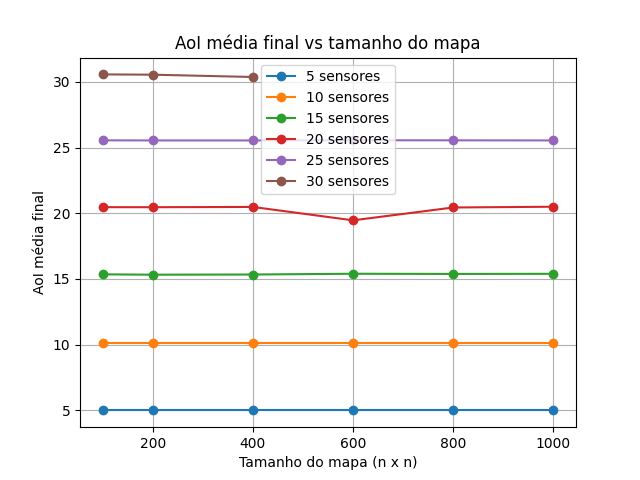
\includegraphics[width=\textwidth]{figs/anafi_aoi_vs_map.png}
    \caption{Parrot Anafi USA}
  \end{subfigure}
  \caption{AoI média final em função do tamanho do mapa.}
  \label{fig:aoi_vs_map}
\end{figure}

A distância total percorrida (Figura~\ref{fig:distance_vs_map}) acompanha o crescimento de $L$ em ambos os modelos e apresenta comportamento inverso em relação a $n_s$ em mapas grandes: mais sensores na mesma área reduzem as distâncias médias entre vizinhos, resultando em rotas mais curtas. Em mapas pequenos ($L \leq 200$\,m), esse efeito é menos pronunciado, pois mesmo com poucos sensores as distâncias entre nós já são curtas.

\begin{figure}[htbp]
  \centering
  \begin{subfigure}[t]{0.49\textwidth}
    \centering
    
\includegraphics[width=\textwidth]{figs/distance_vs_map.png}
    \caption{DJI Matrice 300 RTK}
  \end{subfigure}
  \hfill
  \begin{subfigure}[t]{0.49\textwidth}
    \centering
    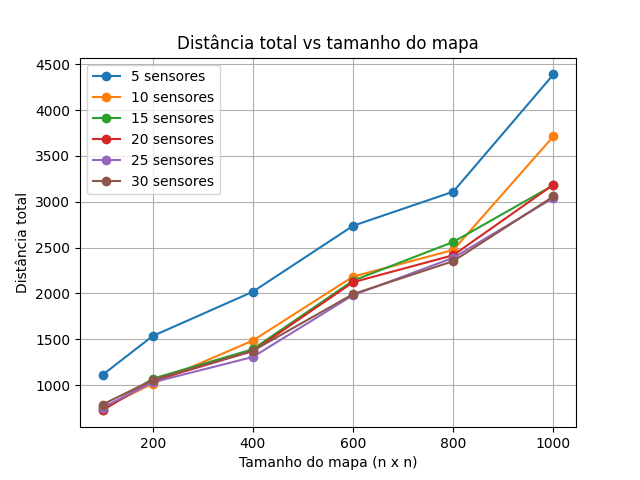
\includegraphics[width=\textwidth]{figs/anafi_distance_vs_map.png}
    \caption{Parrot Anafi USA}
  \end{subfigure}
  \caption{Distância total média em função do tamanho do mapa.}
  \label{fig:distance_vs_map}
\end{figure}

O consumo de energia (Figura~\ref{fig:energy_vs_map}) acompanha o aumento da área: quanto maior $L$, maiores as distâncias entre nós e, portanto, o custo energético de cada aresta. No DJI, o crescimento com $L$ é acentuado, com aparência aproximadamente exponencial na faixa avaliada, consequência de o custo por deslocamento crescer de forma super-linear com a distância percorrida em um único \textit{slot}. No Anafi, o crescimento também é pronunciado e apresenta dois saltos distintos, entre $L=400$ e $600$\,m e entre $L=600$ e $800$\,m. Observa-se ainda um comportamento não-monotônico em $L=1000$\,m: a energia do cenário com $n_s=5$ ($\approx$118\,kJ) supera a dos cenários com $n_s=10$ ($\approx$100\,kJ) e $n_s=15$ ($\approx$76\,kJ), pois, com apenas cinco sensores espalhados em 1000×1000\,m, as distâncias entre nós são maiores do que em cenários mais densos, tornando o roteamento mais custoso.

\begin{figure}[htbp]
  \centering
  \begin{subfigure}[t]{0.49\textwidth}
    \centering
    
\includegraphics[width=\textwidth]{figs/energy_vs_map.png}
    \caption{DJI Matrice 300 RTK}
  \end{subfigure}
  \hfill
  \begin{subfigure}[t]{0.49\textwidth}
    \centering
    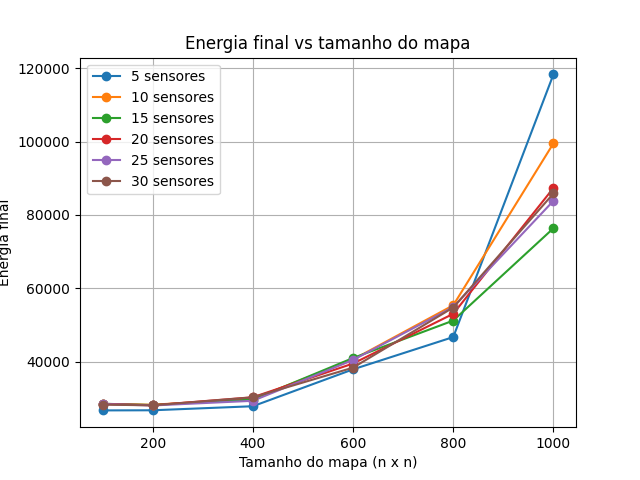
\includegraphics[width=\textwidth]{figs/anafi_energy_vs_map.png}
    \caption{Parrot Anafi USA}
  \end{subfigure}
  \caption{Energia média consumida em função do tamanho do mapa.}
  \label{fig:energy_vs_map}
\end{figure}

\subsection{Comparação com Heurísticas}
\label{sec:comparacao-heuristicas}

Para avaliar o desempenho do modelo de otimização (aqui chamado de MILP, resolvido via Gurobi) em relação a estratégias de baixo custo computacional, foram implementadas três heurísticas construtivas, todas avaliadas sobre os mesmos 36 cenários e as mesmas posições de sensores do Parrot Anafi USA, com 30 rodadas cada:

\begin{itemize}
\item \textbf{Nearest Neighbor (NN)}: a cada passo, o VANT visita o sensor viável (dentro do orçamento de bateria e \textit{slots}) mais próximo da posição atual.
\item \textbf{AoI-Greedy}: a cada passo, visita o sensor de maior AoI ainda viável, com desempate por proximidade. É a heurística mais alinhada ao objetivo de maximizar a AoI coletada.
\item \textbf{Score-Greedy}: a cada passo, visita o sensor de maior razão AoI/distância ainda viável, com desempate por proximidade. Pondera urgência e custo de deslocamento.
\end{itemize}

A Tabela~\ref{tab:cmp-heuristicas} apresenta as médias gerais das cinco métricas sobre todos os cenários. As Figuras~\ref{fig:cmp_all_collected_aoi} a~\ref{fig:cmp_all_energy} detalham, por métrica, o comportamento das quatro estratégias em função do tamanho do mapa, com os cenários separados por faixa de densidade em cada subfigura (a: 5 e 10 sensores; b: 15 e 20; c: 25 e 30).

\begin{table}[htbp]
  \centering
  \caption{Médias gerais das quatro estratégias sobre os 36 cenários (30 rodadas cada) -- Parrot Anafi USA. Para AoI coletada e sensores visitados, maior é melhor. Para AoI média final, energia e distância, menor é melhor.}
  \label{tab:cmp-heuristicas}
  \begin{tabular}{l r r r r}
    \toprule
    \textbf{Métrica} & \textbf{MILP} & \textbf{NN} & \textbf{AoI-Greedy} & \textbf{Score-Greedy} \\
    \midrule
    AoI coletada por rodada      & 309,7  & 145,4   & 298,5  & 300,5 \\
    AoI média final              & 17,8   & 127,2   & 29,5   & 28,5 \\
    Energia final (J)            & 44.943 & 48.711  & 64.571 & 57.738 \\
    Distância total (m)          & 1.933  & 1.272   & 1.719  & 1.502 \\
    Sensores visitados           & 8,33   & 8,22    & 8,19   & 8,24 \\
    \bottomrule
  \end{tabular}
\end{table}

A AoI coletada por rodada (Figura~\ref{fig:cmp_all_collected_aoi}) mede quanta informação desatualizada cada estratégia recolhe ao longo da missão. As heurísticas AoI-Greedy e Score-Greedy, construídas em torno do mesmo objetivo do MILP, aproximam-se muito do modelo ótimo: a AoI-Greedy fica a apenas $-3{,}6\%$ (298,5 contra 309,7) e a Score-Greedy a $-3{,}0\%$ (300,5). O NN coleta bem menos ($145,4$, menos da metade do MILP) e degrada sobretudo em mapas grandes com poucos sensores: nos cenários de 5 e 10 sensores (Figura~\ref{fig:cmp_collected_a}), sua curva despenca à medida que $L$ cresce, enquanto o MILP se mantém estável. Com o aumento da densidade (Figuras~\ref{fig:cmp_collected_b} e~\ref{fig:cmp_collected_c}), a diferença entre as estratégias diminui, pois há mais sensores próximos disponíveis para coleta.

\begin{figure}[htbp]
  \centering
  \begin{subfigure}{0.8\textwidth}
    \centering
    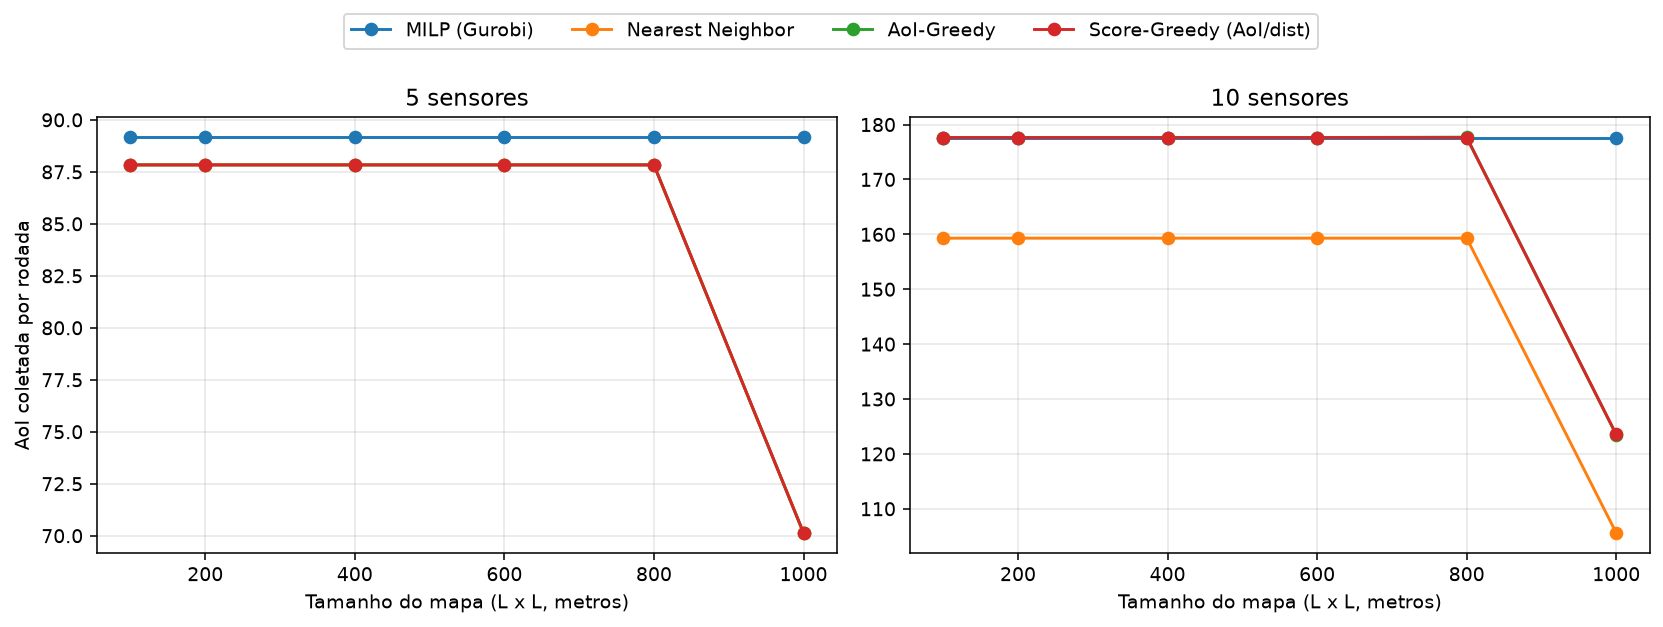
\includegraphics[width=\textwidth]{figs/cmp_all_collected_aoi_p1.png}
    \caption{5 e 10 sensores}
    \label{fig:cmp_collected_a}
  \end{subfigure}

  \begin{subfigure}{0.8\textwidth}
    \centering
    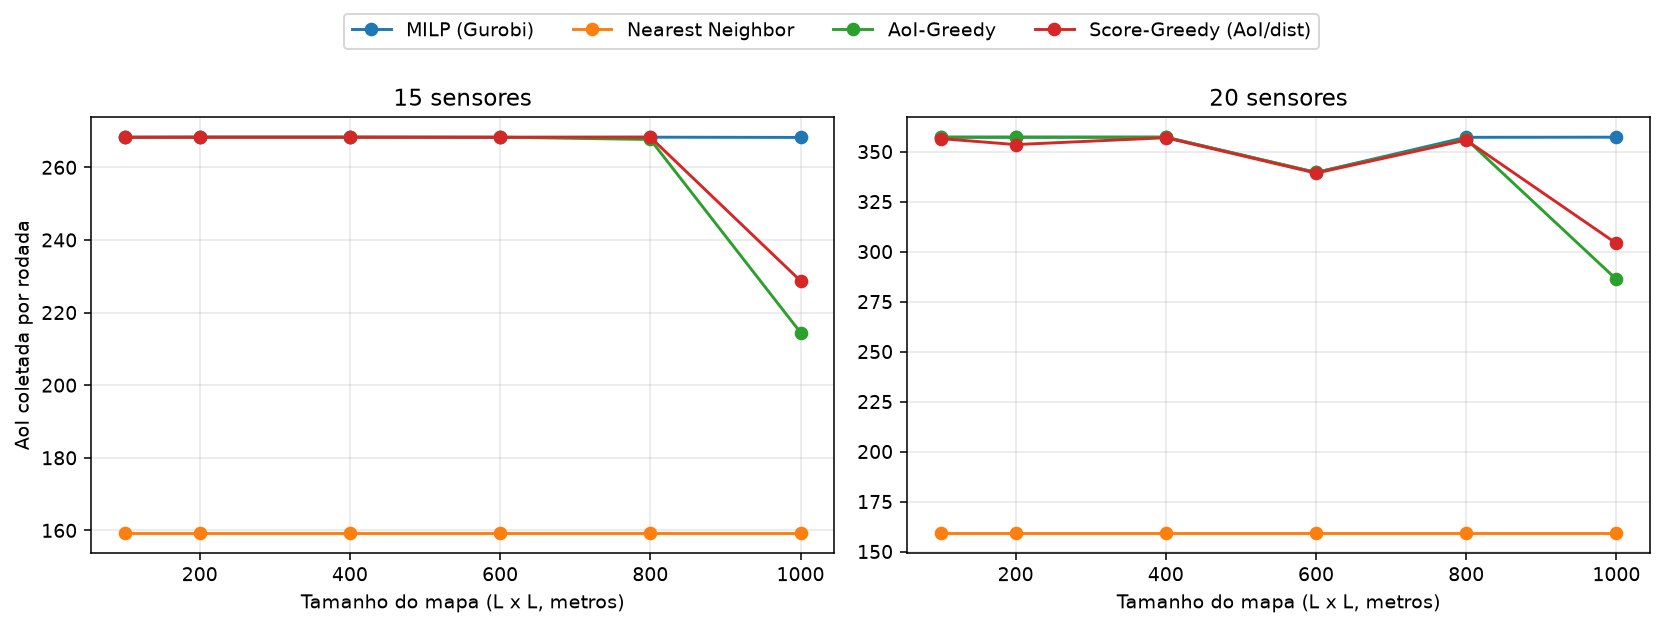
\includegraphics[width=\textwidth]{figs/cmp_all_collected_aoi_p2.png}
    \caption{15 e 20 sensores}
    \label{fig:cmp_collected_b}
  \end{subfigure}

  \begin{subfigure}{0.8\textwidth}
    \centering
    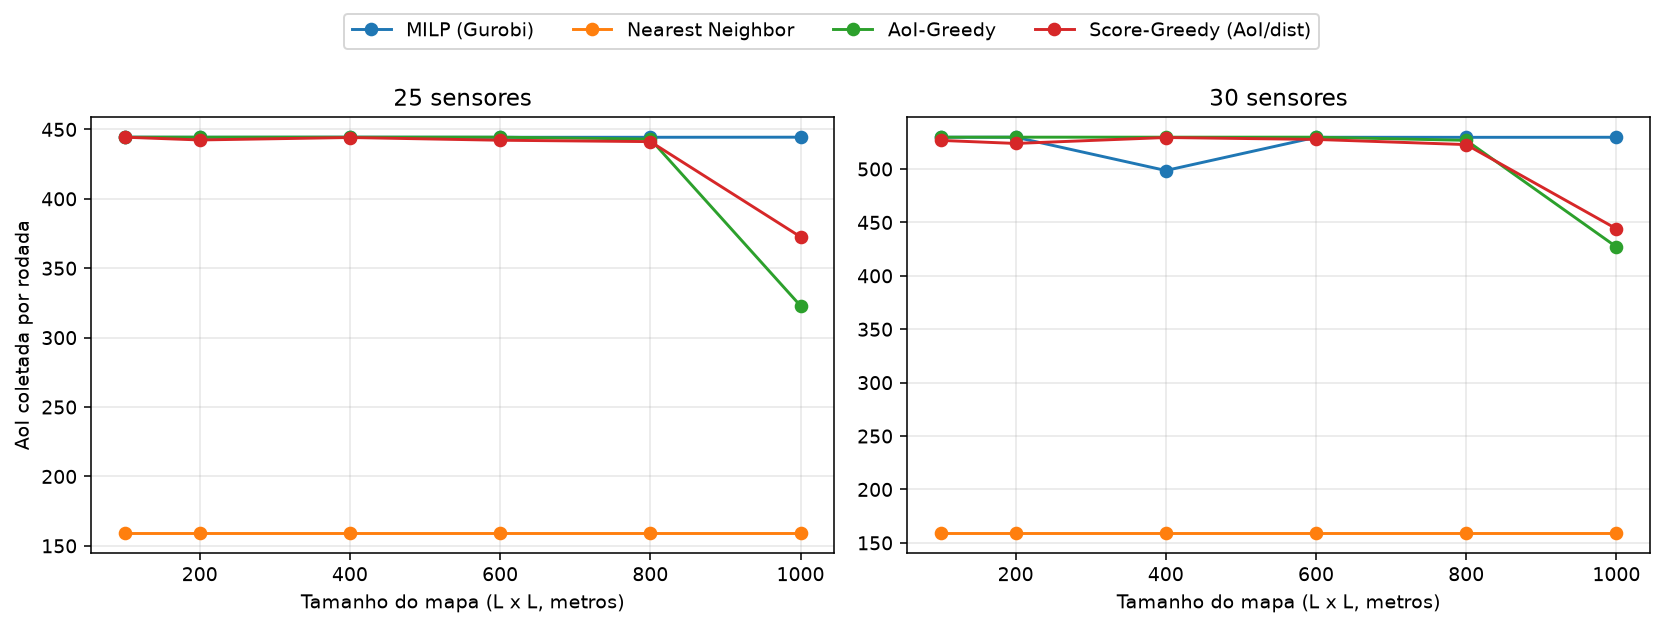
\includegraphics[width=\textwidth]{figs/cmp_all_collected_aoi_p3.png}
    \caption{25 e 30 sensores}
    \label{fig:cmp_collected_c}
  \end{subfigure}
  \caption{AoI coletada por rodada em função do tamanho do mapa, para as quatro estratégias.}
  \label{fig:cmp_all_collected_aoi}
\end{figure}

A AoI média final (Figura~\ref{fig:cmp_all_avg_final_aoi}) mede quão atualizados ficam os dados ao término da missão. O MILP entrega a menor idade residual (17,8), seguido de perto pela Score-Greedy (28,5) e pela AoI-Greedy (29,5), ambas cerca de $38$ a $40\%$ acima do MILP, porém muito melhores que o NN, que é o pior por larga margem (127,2). O contraste aparece com mais nitidez nos cenários de baixa densidade (Figura~\ref{fig:cmp_avg_a}), em que a curva do NN se descola das demais, refletindo sua incapacidade de manter a rede atualizada quando os sensores estão distantes.

\begin{figure}[htbp]
  \centering
  \begin{subfigure}{0.8\textwidth}
    \centering
    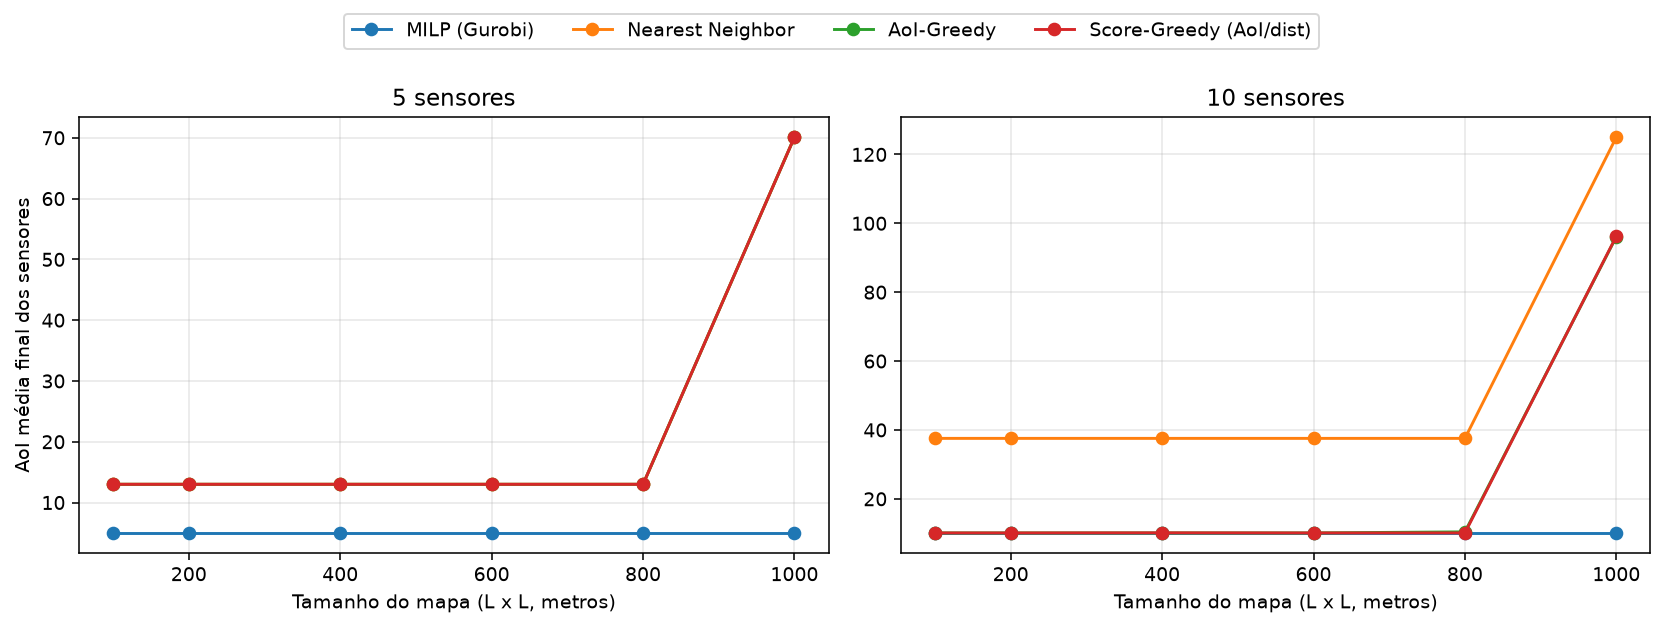
\includegraphics[width=\textwidth]{figs/cmp_all_avg_final_aoi_p1.png}
    \caption{5 e 10 sensores}
    \label{fig:cmp_avg_a}
  \end{subfigure}

  \begin{subfigure}{0.8\textwidth}
    \centering
    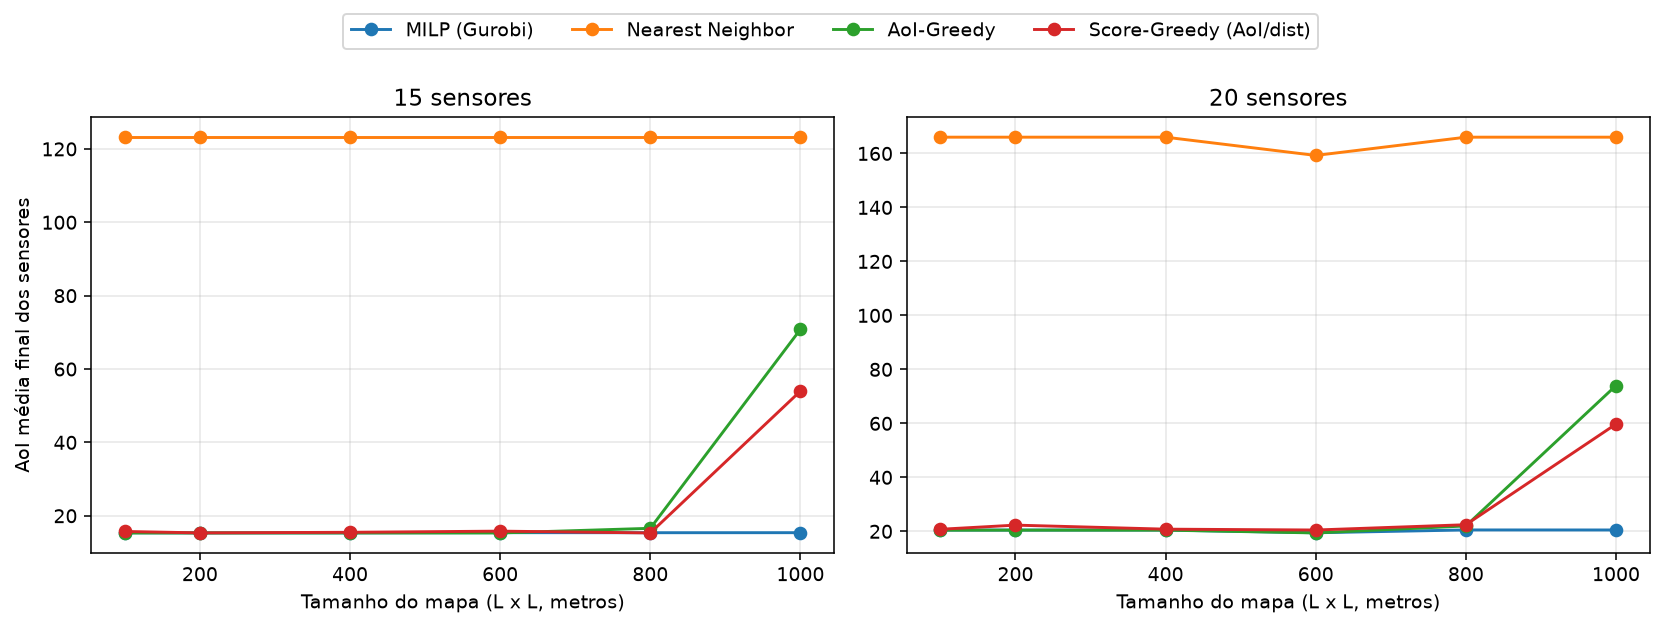
\includegraphics[width=\textwidth]{figs/cmp_all_avg_final_aoi_p2.png}
    \caption{15 e 20 sensores}
    \label{fig:cmp_avg_b}
  \end{subfigure}

  \begin{subfigure}{0.8\textwidth}
    \centering
    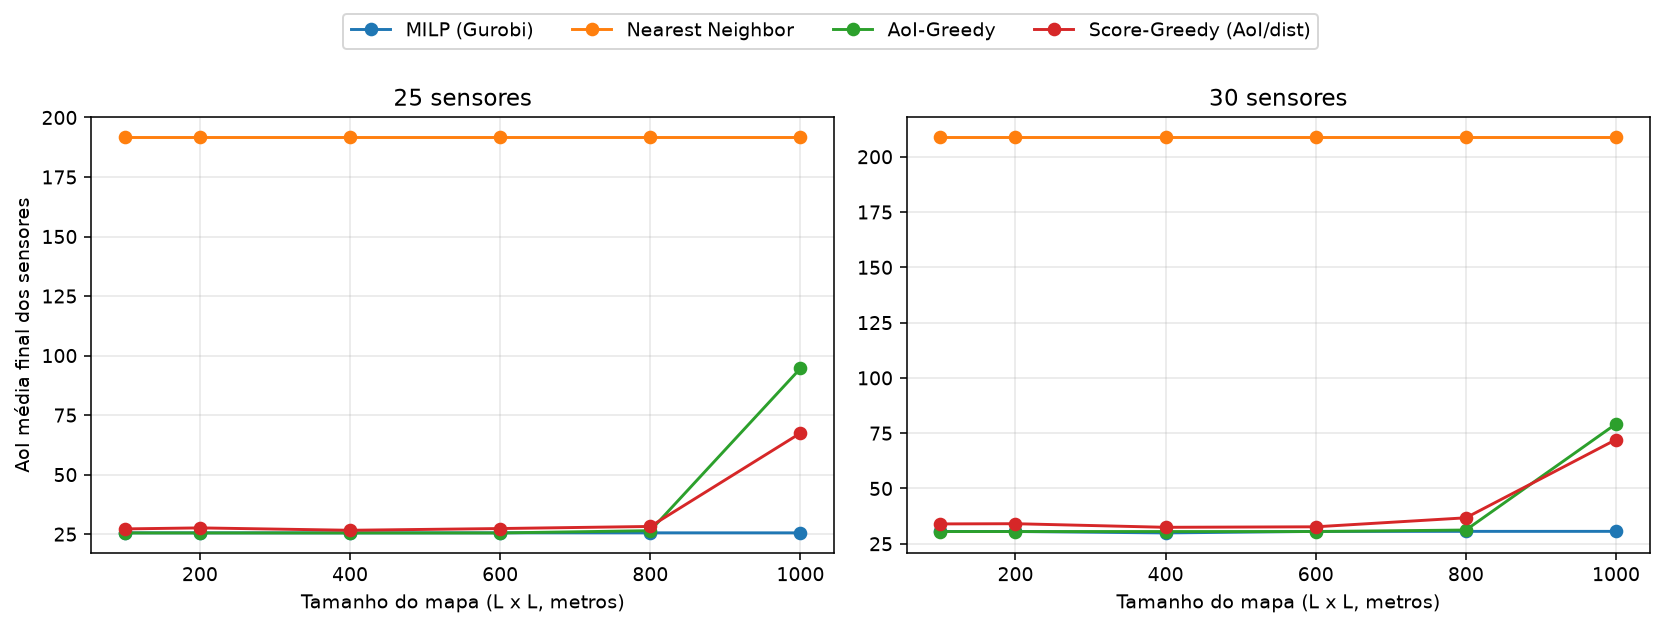
\includegraphics[width=\textwidth]{figs/cmp_all_avg_final_aoi_p3.png}
    \caption{25 e 30 sensores}
    \label{fig:cmp_avg_c}
  \end{subfigure}
  \caption{AoI média final dos sensores em função do tamanho do mapa, para as quatro estratégias.}
  \label{fig:cmp_all_avg_final_aoi}
\end{figure}

O consumo de energia (Figura~\ref{fig:cmp_all_energy}) evidencia o ponto fraco das heurísticas gulosas por AoI: a AoI-Greedy gasta $+43{,}7\%$ (64.571\,J contra 44.943\,J do MILP) e a Score-Greedy $+28{,}5\%$ (57.738\,J), pois maximizam a AoI sem ponderar adequadamente o custo do deslocamento. O NN consome pouco (48.711\,J, apenas $+7{,}7\%$ sobre o MILP), mas à custa de coletar pouco. A vantagem de ponderar a distância fica clara na comparação entre as duas gulosas: a Score-Greedy domina a AoI-Greedy, coletando essencialmente a mesma AoI ($+0{,}7\%$) com $-10{,}6\%$ de energia e $-12{,}6\%$ de distância. Em todas as estratégias, o consumo cresce de forma acentuada com $L$ (Figuras~\ref{fig:cmp_energy_a} a~\ref{fig:cmp_energy_c}).

\begin{figure}[htbp]
  \centering
  \begin{subfigure}{0.8\textwidth}
    \centering
    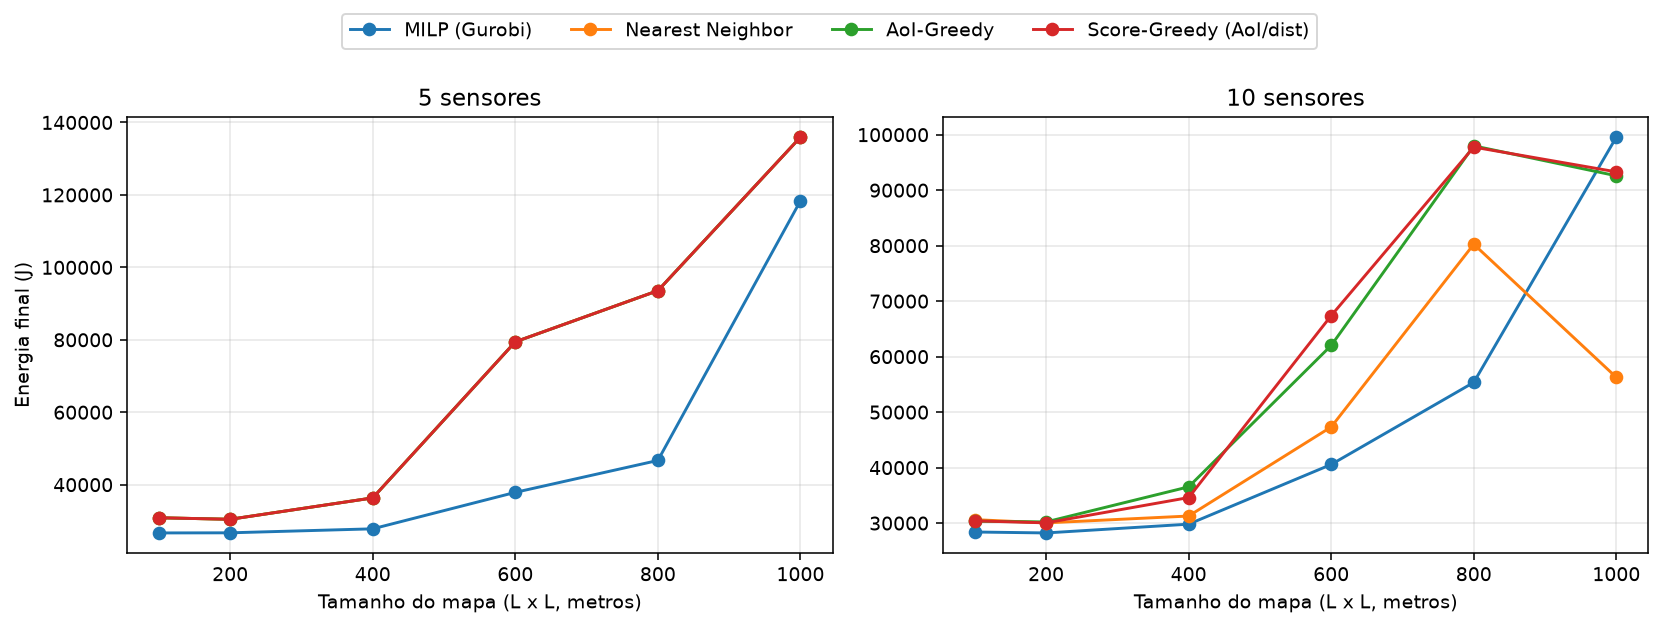
\includegraphics[width=\textwidth]{figs/cmp_all_energy_p1.png}
    \caption{5 e 10 sensores}
    \label{fig:cmp_energy_a}
  \end{subfigure}

  \begin{subfigure}{0.8\textwidth}
    \centering
    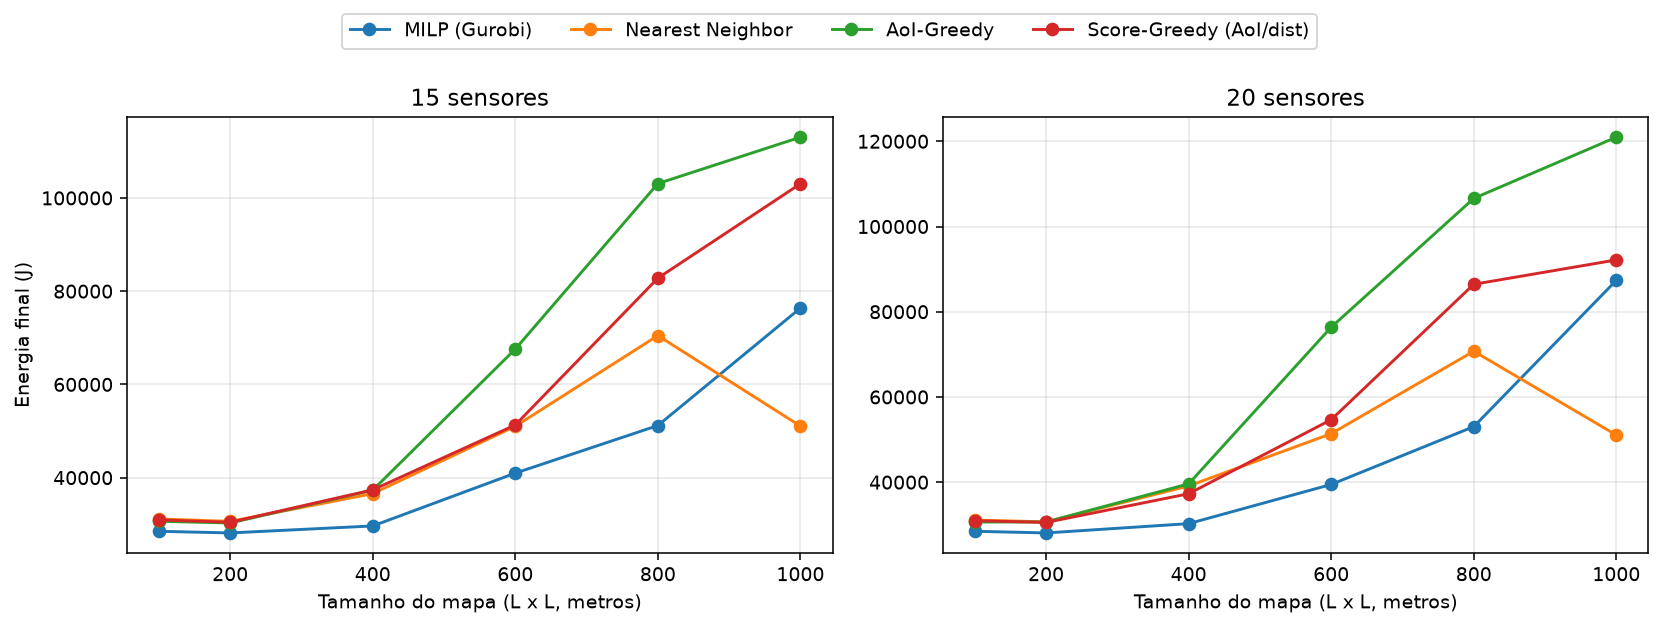
\includegraphics[width=\textwidth]{figs/cmp_all_energy_p2.png}
    \caption{15 e 20 sensores}
    \label{fig:cmp_energy_b}
  \end{subfigure}

  \begin{subfigure}{0.8\textwidth}
    \centering
    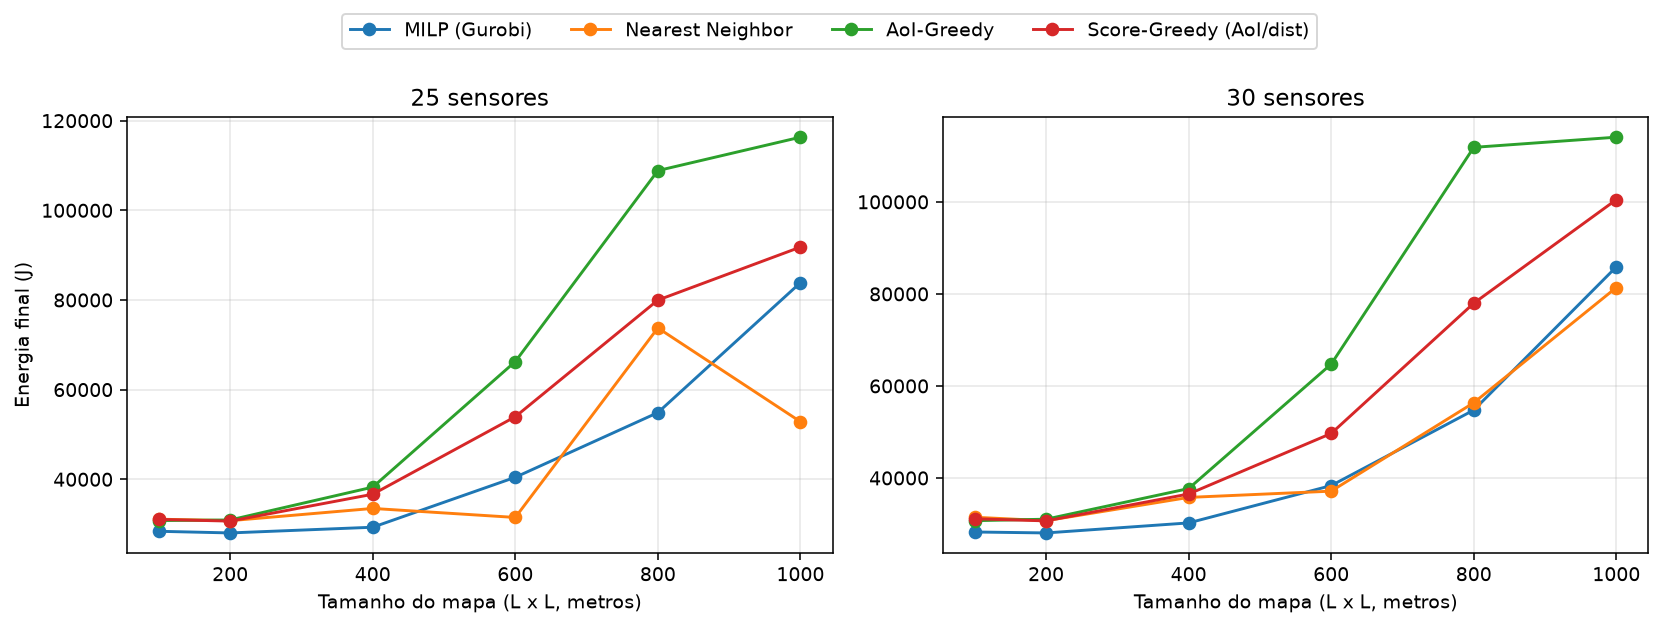
\includegraphics[width=\textwidth]{figs/cmp_all_energy_p3.png}
    \caption{25 e 30 sensores}
    \label{fig:cmp_energy_c}
  \end{subfigure}
  \caption{Energia final consumida em função do tamanho do mapa, para as quatro estratégias.}
  \label{fig:cmp_all_energy}
\end{figure}

Em síntese, cada heurística privilegia um aspecto isolado: o NN economiza energia mas coleta pouco e desatualiza a rede, enquanto as gulosas por AoI coletam quase tanto quanto o MILP, porém a um custo energético muito maior. A Score-Greedy é a melhor heurística do conjunto, dominando a AoI-Greedy e sendo a mais próxima do MILP, mas ainda assim permanece $28{,}5\%$ acima dele em energia. Isso evidencia o valor da formulação exata: por ser multiobjetivo lexicográfica (maximiza a AoI coletada e, em seguida, minimiza a energia entre as soluções de AoI ótima), o MILP é a única estratégia que alcança, ao mesmo tempo, a maior AoI coletada e o menor consumo energético.

\subsection{Variante com Revisitas}

Com base nos resultados do modelo base, investigou-se uma variante que relaxa a restrição de visita única por sensor: o modelo com revisitas (\textit{revisit}). Nessa configuração, o VANT pode visitar o mesmo sensor mais de uma vez durante uma missão, com o objetivo de coletar AoI adicional de sensores de alto valor nas rodadas em que a AoI acumulada é elevada.

\subsubsection{Implementação}
A modificação consiste na substituição da restrição de visita única (Equação~\eqref{eq:visita-unica}), $\sum_t v_{j,t} \leq 1$, por $\sum_t v_{j,t} \leq K$, onde $K$ é o número máximo de revisitas permitido por sensor por missão. O parâmetro $K$ é configurável via argumento de linha de comando (\texttt{--max-revisits}). Nos experimentos desta seção, adotou-se $K = 3$.

\subsubsection{Desafios computacionais}
A adoção de revisitas amplia consideravelmente o espaço de soluções viáveis do modelo MILP. Com $K = 3$, o número de combinações possíveis de padrões de visita cresce exponencialmente, tornando a exploração da árvore de \textit{branch-and-bound} pelo Gurobi significativamente mais custosa em memória. Em cenários com $n_s \geq 20$ e $L \geq 600$\,m, o processo de otimização chegou a consumir vários gigabytes de RAM, causando instabilidades no ambiente de execução.

Para contornar esses problemas, foram adotadas três medidas: (i) limitação do número de \textit{threads} do Gurobi a 2, reduzindo o paralelismo da exploração da árvore, (ii) ativação do parâmetro \texttt{NodefileStart = 0.5\,GB}, que instrui o solver a descarregar nós da árvore para disco ao atingir esse limite de memória RAM, e (iii) definição de \texttt{SoftMemLimit = 4\,GB}, que encerra a otimização de forma controlada e retorna a melhor solução encontrada até o momento quando o uso de memória ultrapassa esse valor. Adicionalmente, rodadas em que o solver não encontrou solução viável dentro do limite de tempo ou memória são registradas com métricas zeradas e AoI envelhecida normalmente, garantindo a consistência da cadeia de estado entre rodadas.

\subsubsection{Resultados e comparativo}
Os resultados do modelo com revisitas foram comparados com o modelo base para os mesmos 36 cenários, utilizando as mesmas posições de sensores e os mesmos parâmetros do Parrot Anafi USA.

A análise revela que a variante com revisitas \textbf{não trouxe melhora na qualidade da solução} em termos de AoI. Como mostra a Figura~\ref{fig:cmp_aoi_vs_map}, as curvas do modelo base e da variante com revisitas praticamente se sobrepõem em todas as faixas de densidade, dos cenários esparsos (Figura~\ref{fig:rev_aoi_a}) aos mais densos (Figura~\ref{fig:rev_aoi_c}). O mapa de variação percentual da AoI (Figura~\ref{fig:delta_aoi}) confirma o quadro: a AoI média final permaneceu estatisticamente equivalente ao modelo base em praticamente todos os cenários, com variações menores que $\pm 3\%$, dentro da margem de ruído das 30 rodadas.

\begin{figure}[htbp]
  \centering
  \begin{subfigure}{0.8\textwidth}
    \centering
    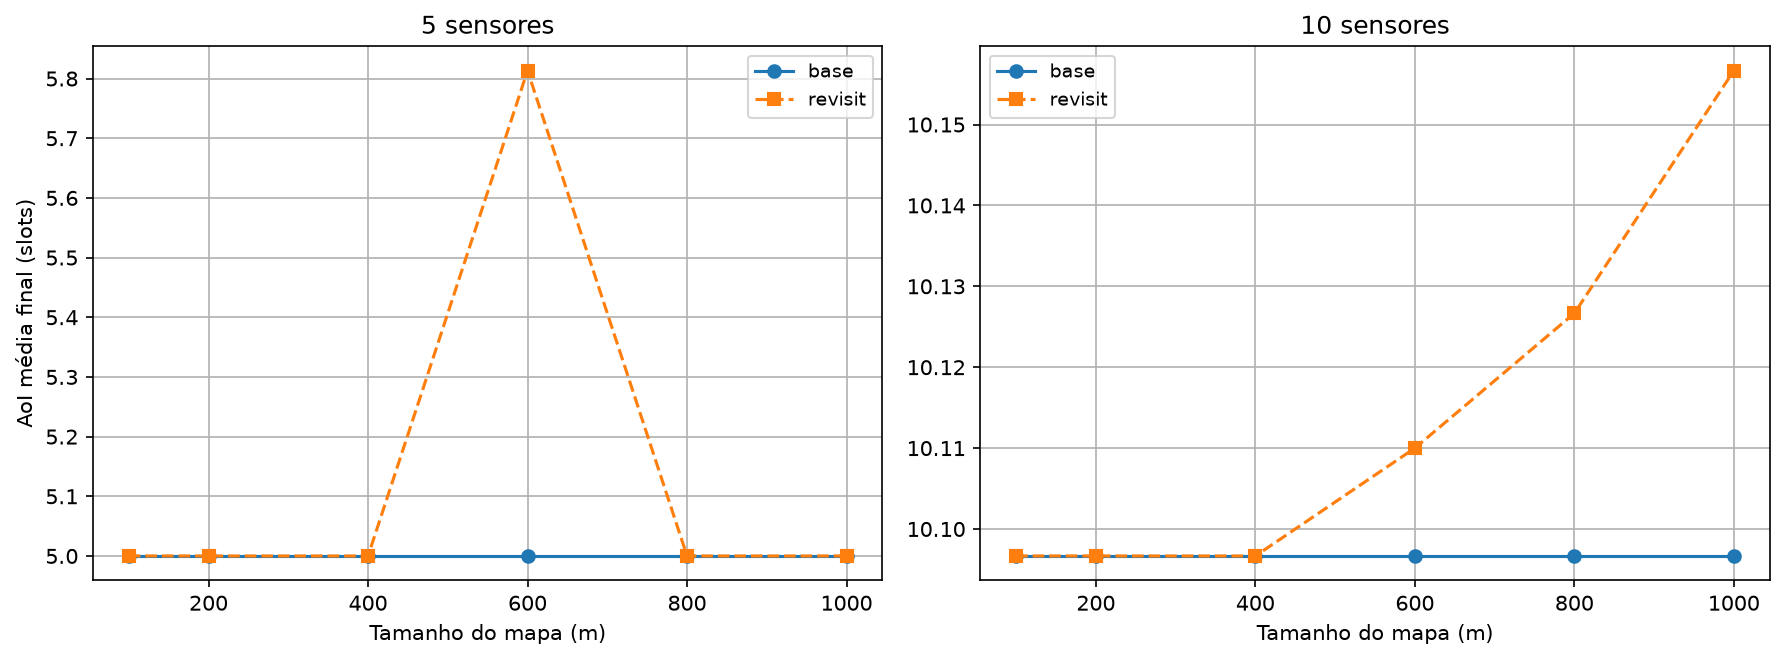
\includegraphics[width=\textwidth]{figs/cmp_aoi_vs_map_p1.png}
    \caption{5 e 10 sensores}
    \label{fig:rev_aoi_a}
  \end{subfigure}

  \begin{subfigure}{0.8\textwidth}
    \centering
    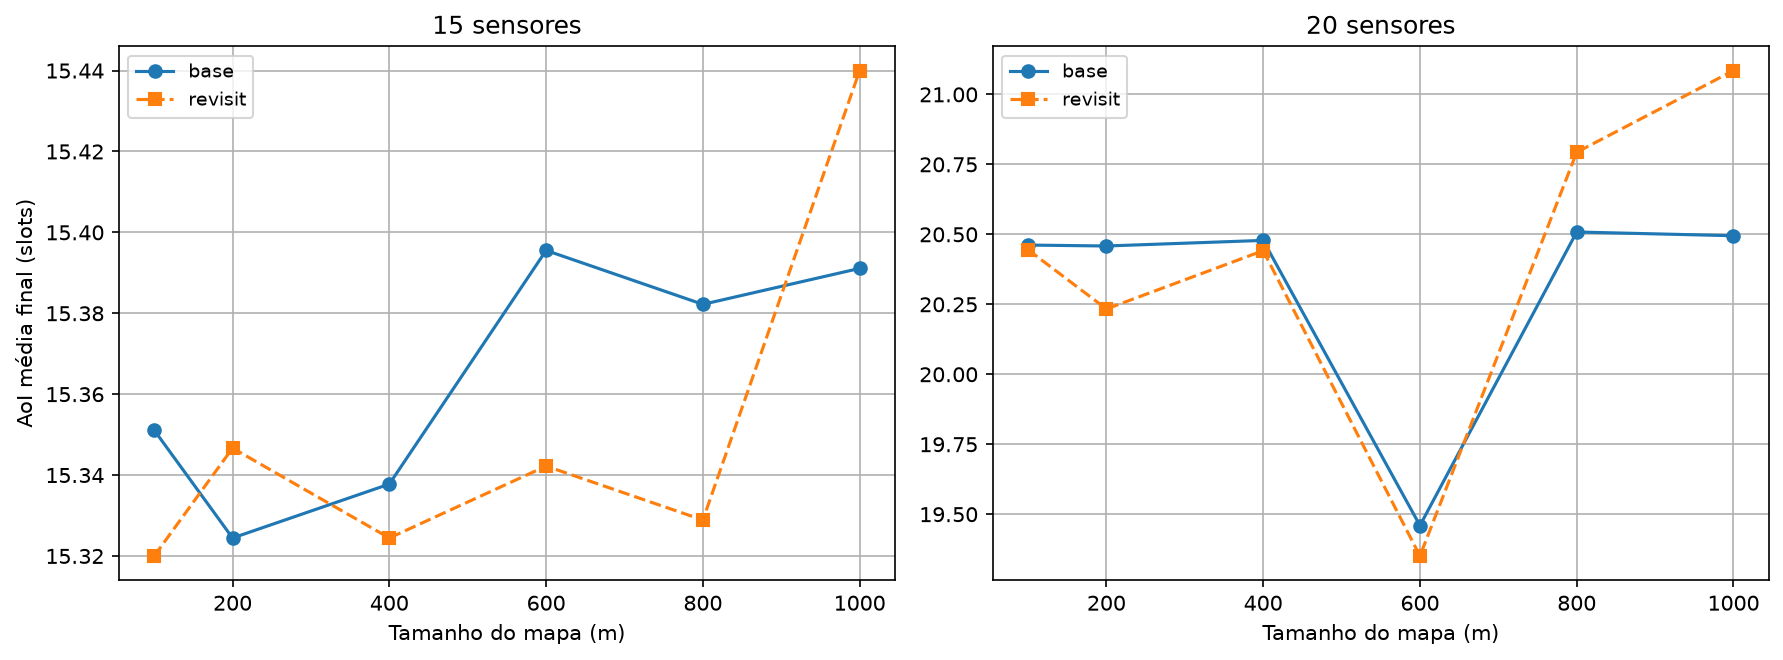
\includegraphics[width=\textwidth]{figs/cmp_aoi_vs_map_p2.png}
    \caption{15 e 20 sensores}
    \label{fig:rev_aoi_b}
  \end{subfigure}

  \begin{subfigure}{0.8\textwidth}
    \centering
    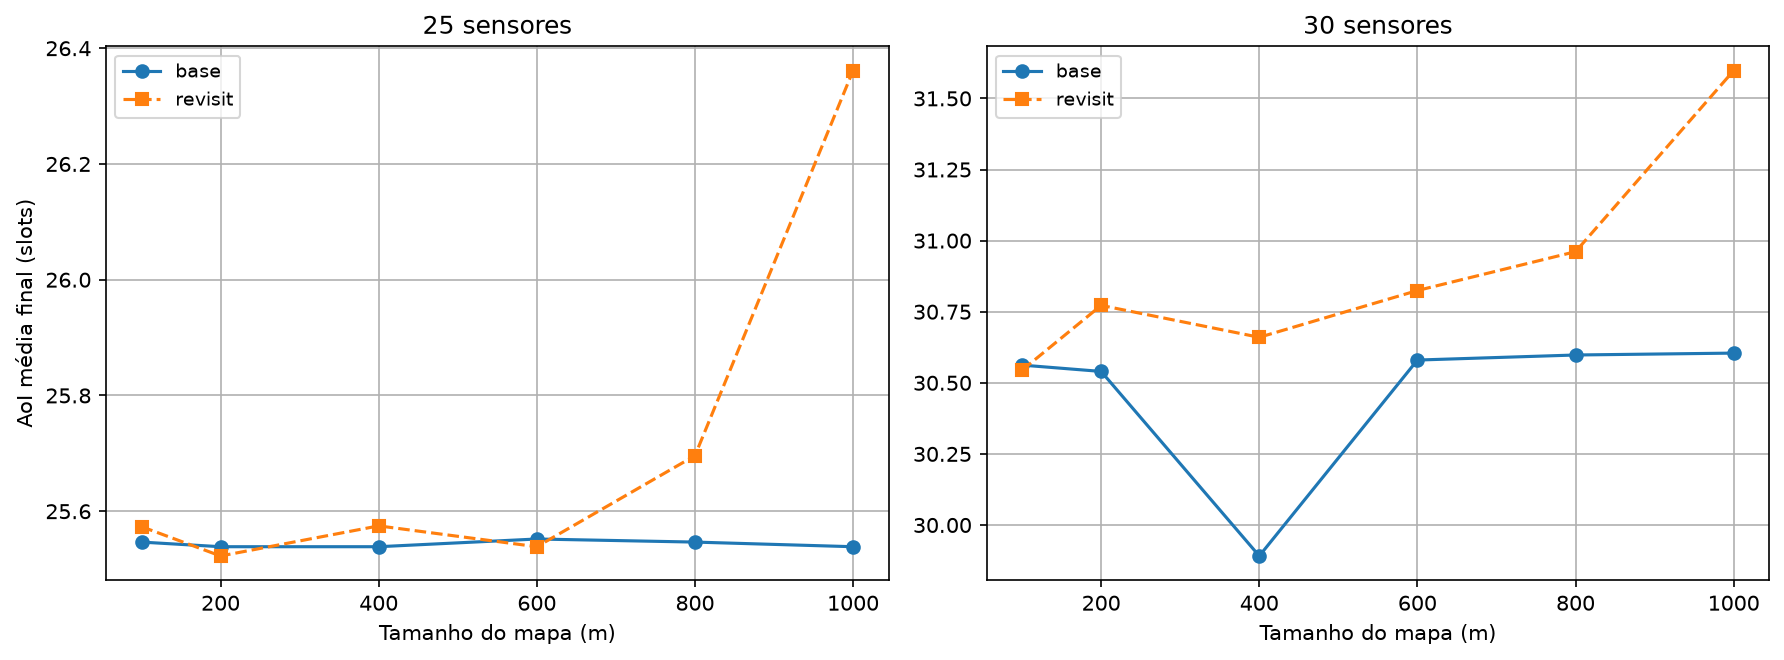
\includegraphics[width=\textwidth]{figs/cmp_aoi_vs_map_p3.png}
    \caption{25 e 30 sensores}
    \label{fig:rev_aoi_c}
  \end{subfigure}
  \caption{AoI média final: comparativo entre o modelo base e a variante com revisitas ($K=3$).}
  \label{fig:cmp_aoi_vs_map}
\end{figure}

Em contrapartida, o consumo energético aumentou substancialmente com as revisitas (Figura~\ref{fig:cmp_energy_vs_map}). Para mapas pequenos ($L \leq 200$\,m), o acréscimo foi modesto ($+3$ a $+6\%$), mas cresce fortemente com a área: entre $+33\%$ e $+45\%$ para $L=400$\,m e entre $+108\%$ e $+189\%$ para $L \geq 600$\,m, efeito que se acentua dos cenários de baixa densidade (Figura~\ref{fig:rev_energy_a}) aos de alta (Figura~\ref{fig:rev_energy_c}) e que o mapa de variação da energia (Figura~\ref{fig:delta_energy}) resume. Em vários cenários com $L \geq 600$\,m, a energia da variante ultrapassou $100$\,kJ, aproximando-se do limite de bateria de $141$\,kJ.

\begin{figure}[htbp]
  \centering
  \begin{subfigure}{0.8\textwidth}
    \centering
    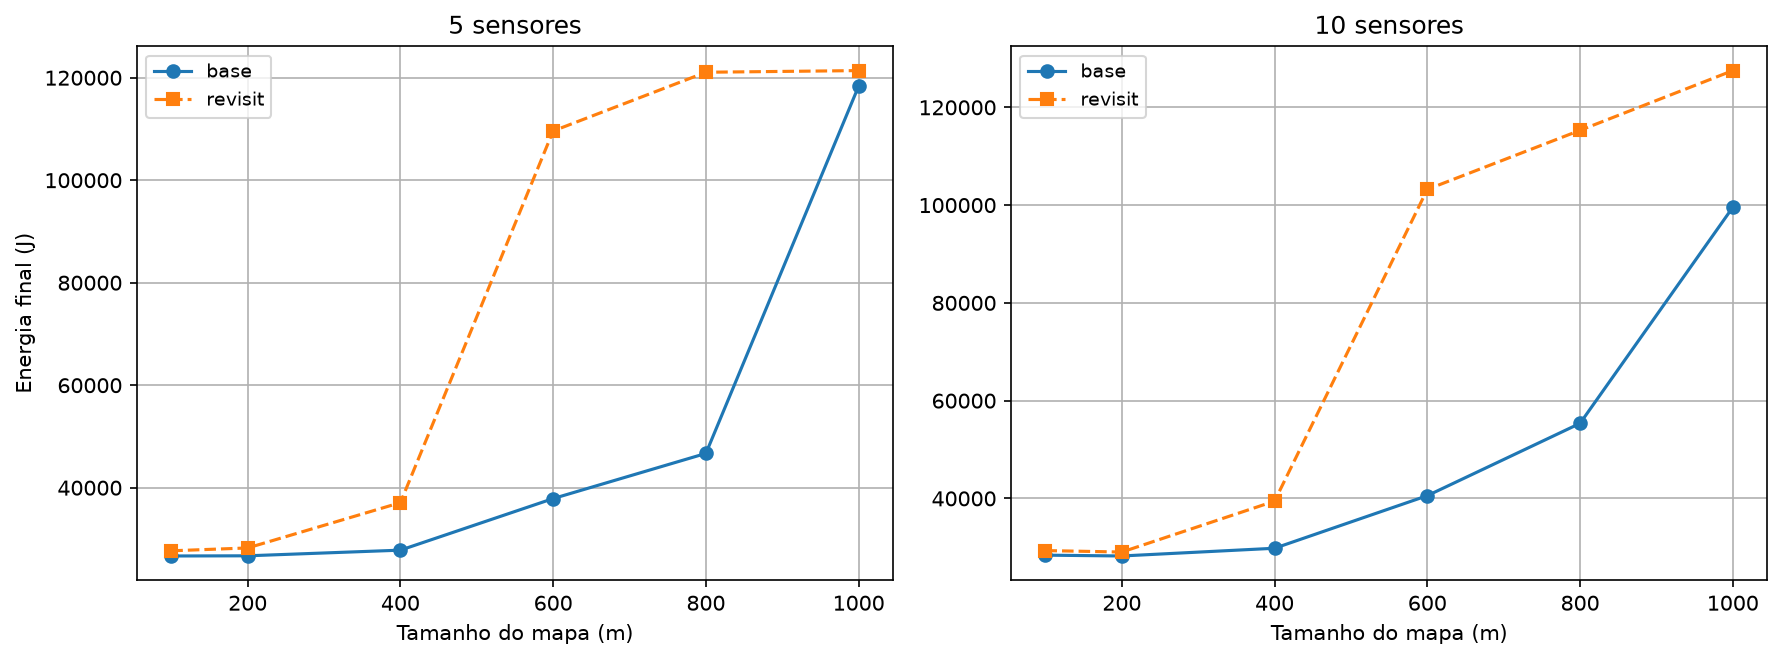
\includegraphics[width=\textwidth]{figs/cmp_energy_vs_map_p1.png}
    \caption{5 e 10 sensores}
    \label{fig:rev_energy_a}
  \end{subfigure}

  \begin{subfigure}{0.8\textwidth}
    \centering
    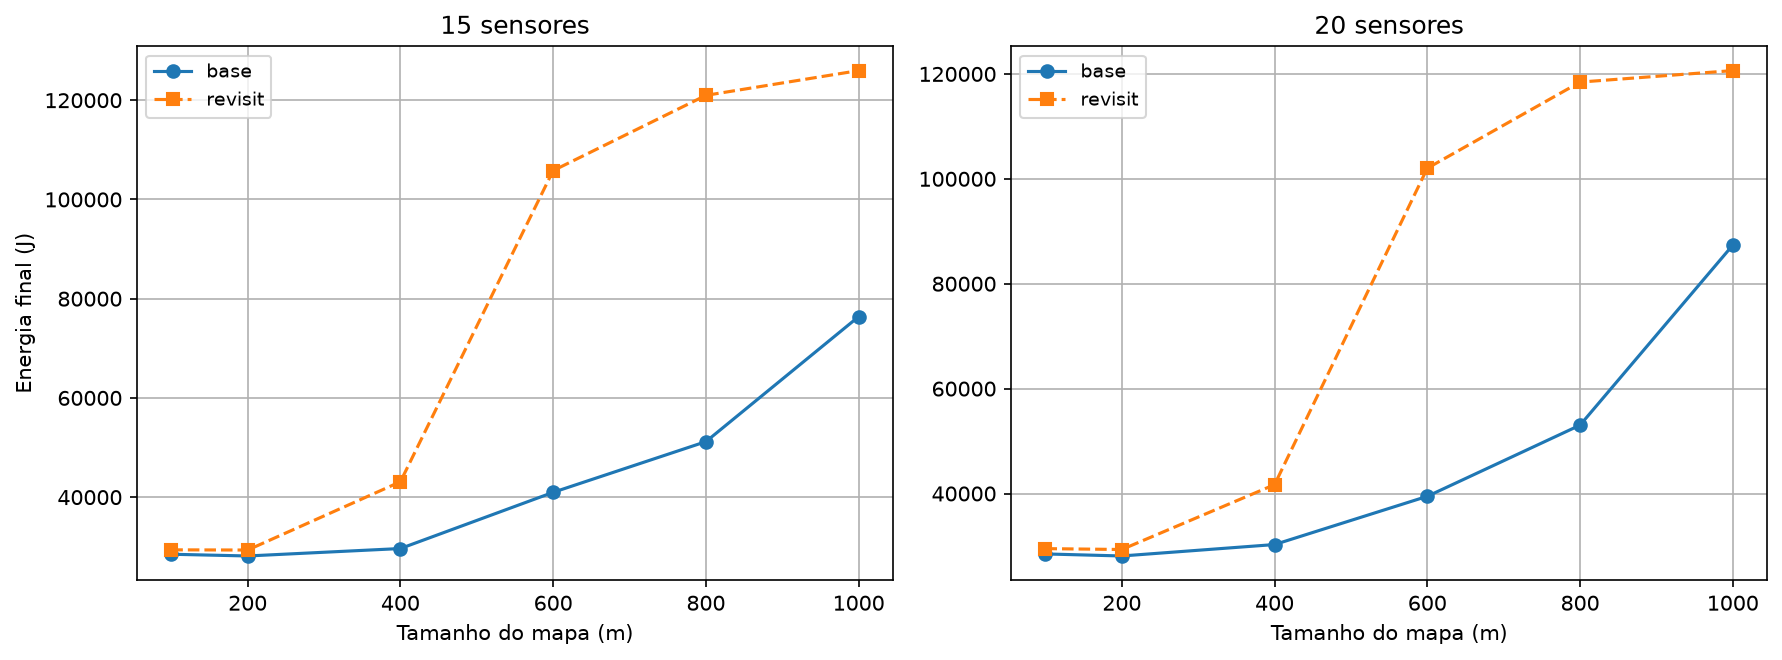
\includegraphics[width=\textwidth]{figs/cmp_energy_vs_map_p2.png}
    \caption{15 e 20 sensores}
    \label{fig:rev_energy_b}
  \end{subfigure}

  \begin{subfigure}{0.8\textwidth}
    \centering
    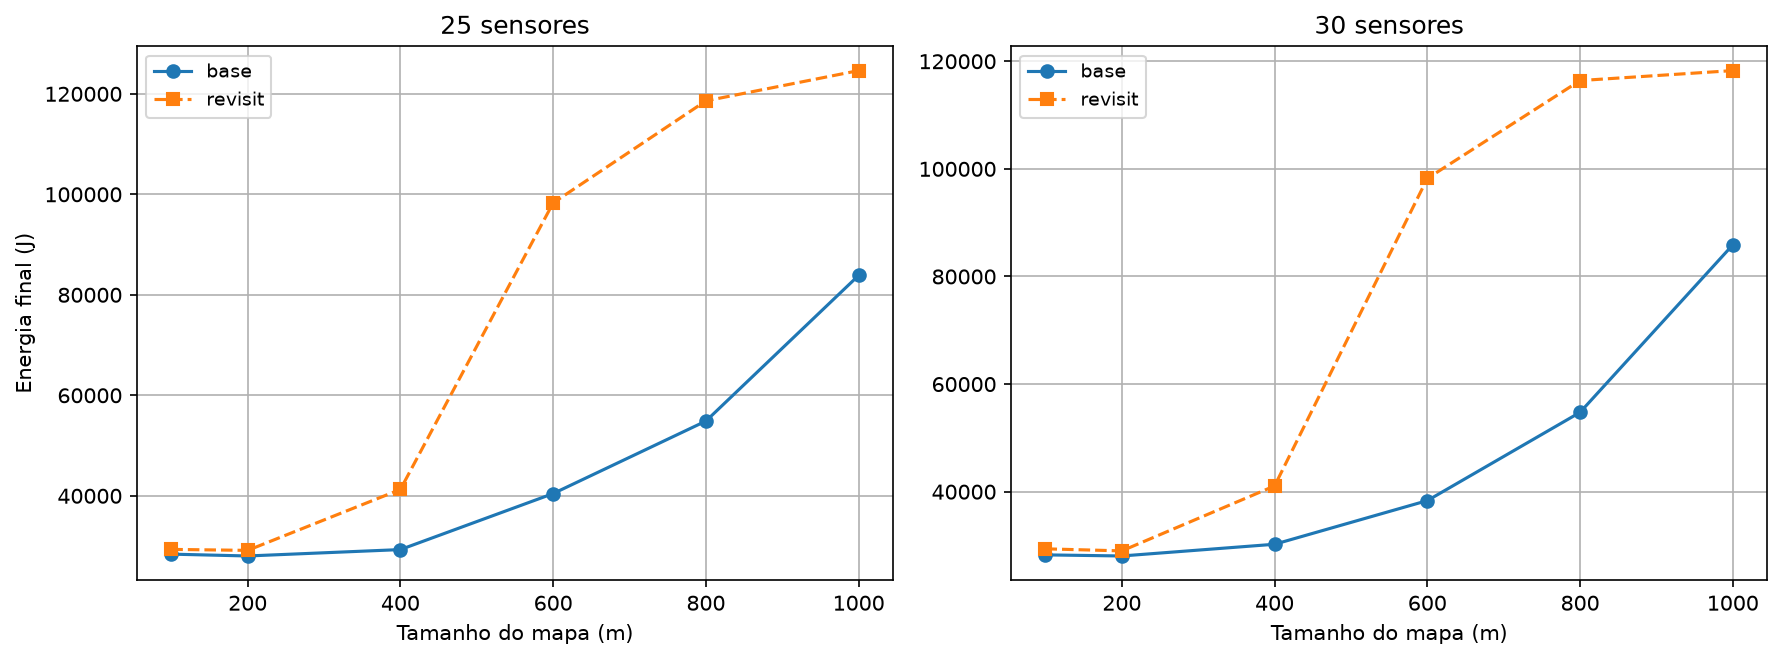
\includegraphics[width=\textwidth]{figs/cmp_energy_vs_map_p3.png}
    \caption{25 e 30 sensores}
    \label{fig:rev_energy_c}
  \end{subfigure}
  \caption{Energia média consumida: comparativo entre o modelo base e a variante com revisitas ($K=3$).}
  \label{fig:cmp_energy_vs_map}
\end{figure}

\begin{figure}[htbp]
  \centering
  \begin{subfigure}[t]{0.49\textwidth}
    \centering
    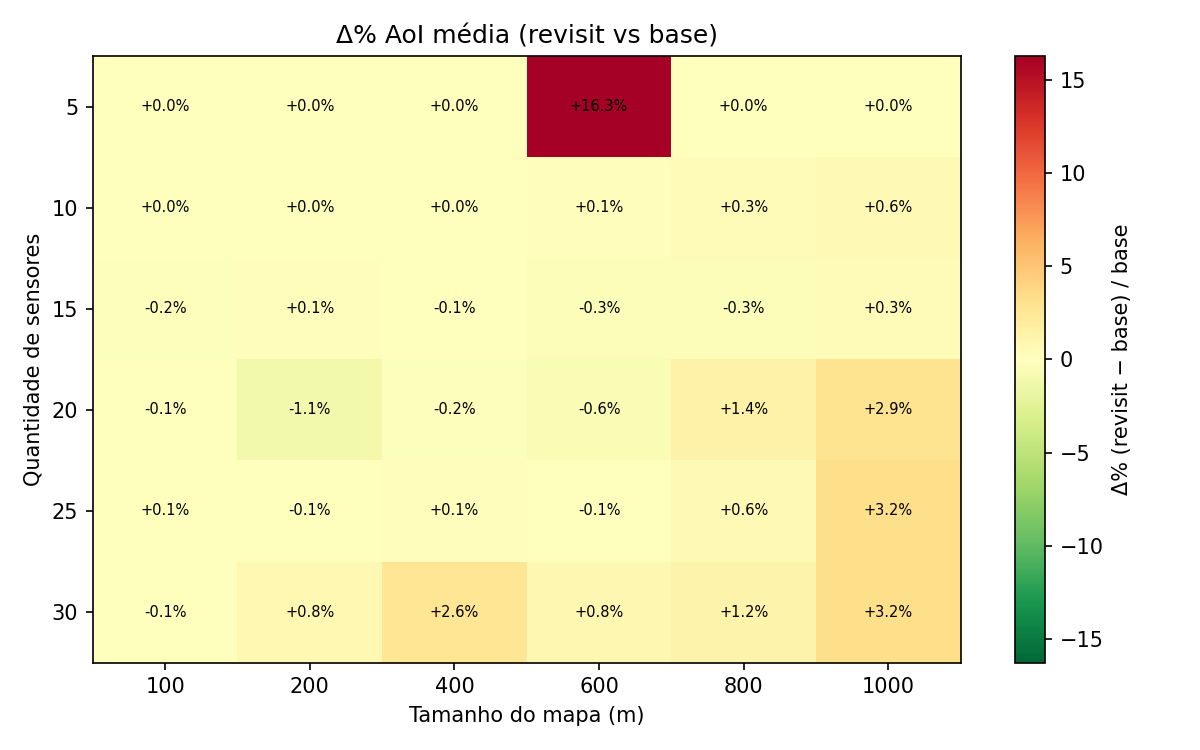
\includegraphics[width=\textwidth]{figs/delta_aoi_heatmap.png}
    \caption{AoI média final}
    \label{fig:delta_aoi}
  \end{subfigure}
  \hfill
  \begin{subfigure}[t]{0.49\textwidth}
    \centering
    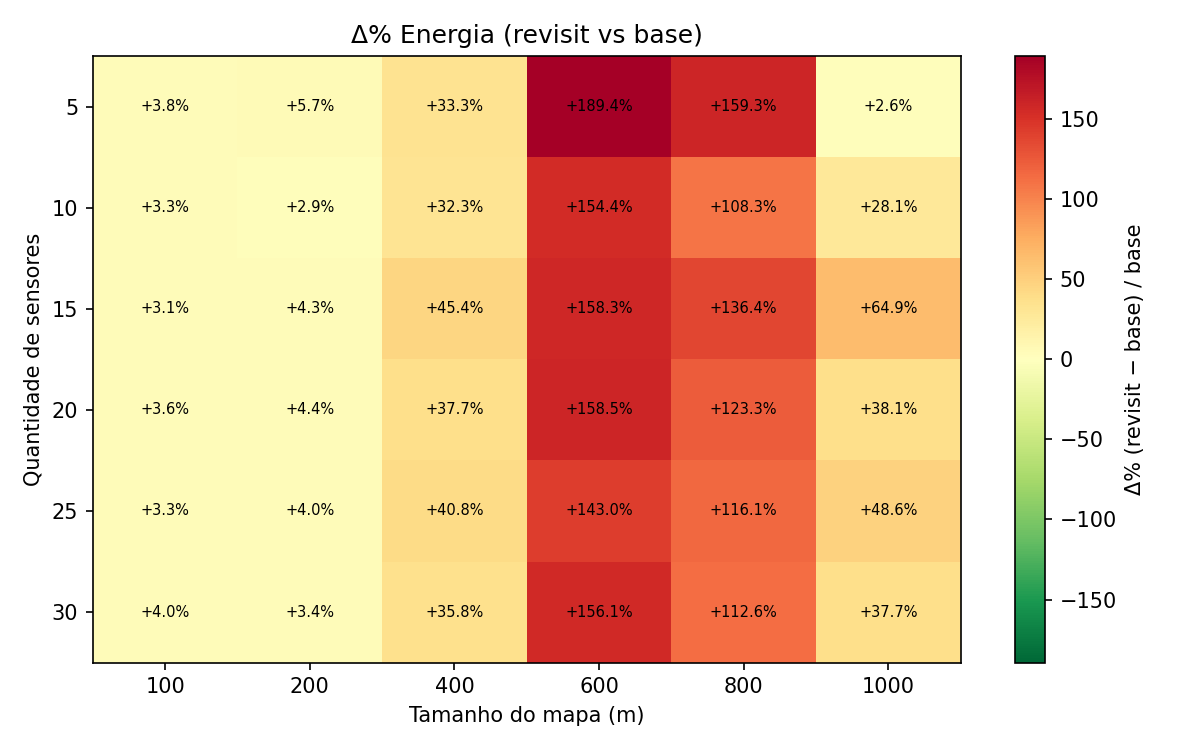
\includegraphics[width=\textwidth]{figs/delta_energy_heatmap.png}
    \caption{Energia consumida}
    \label{fig:delta_energy}
  \end{subfigure}
  \caption{Variação percentual (revisit $-$ base) / base entre a variante com revisitas e o modelo base. Valores positivos indicam piora (aumento).}
  \label{fig:delta_heatmaps}
\end{figure}

Esse comportamento pode ser explicado pela natureza do modelo de otimização: ao permitir revisitas, o solver passa a incluir trajetórias em que o VANT retorna a sensores já visitados para coletar, em um \textit{slot} posterior, a AoI que eles voltaram a acumular desde a visita anterior, mas esse ganho marginal de AoI não compensa o custo energético do deslocamento adicional. Com $K=3$, o orçamento de tempo pairado disponível é distribuído em menos sensores distintos, reduzindo a diversidade de coleta e, consequentemente, sem benefício líquido para a AoI média da rede.

Conclui-se que, para a configuração estudada ($K=3$, 20 slots de 10\,s, Parrot Anafi USA), a restrição de visita única é uma escolha eficiente: ela força o otimizador a diversificar as visitas, obtendo qualidade de AoI equivalente a um custo energético significativamente menor.

\subsection{Escala espacial e o papel das heurísticas}
\label{sec:escala-heuristicas}

Os experimentos apresentados restringiram-se a áreas de até $1000\times1000$\,m. Essa escolha decorre da discretização adotada no modelo de energia (Capítulo~\ref{sec:modelagem}): como cada transição entre nós é concluída em um único \textit{slot} de duração fixa $\Delta t = 10$\,s, áreas maiores implicariam velocidades nominais irrealistas e, com frequência, um custo energético por deslocamento superior à própria capacidade da bateria, tornando o cenário fisicamente inviável sob essa parametrização.

As heurísticas construtivas, por si só, não são o fator limitante: elas podem ser executadas em áreas maiores sem dificuldade. Para tornar tais áreas energeticamente viáveis, entretanto, seria necessário aumentar a duração do \textit{slot} $\Delta t$, permitindo velocidades menores e um custo de deslocamento compatível com a bateria. Esse ajuste, porém, altera a base temporal do experimento e inviabiliza a comparação direta com os cenários menores, que adotam $\Delta t = 10$\,s. Além disso, um $\Delta t$ maior é contraproducente no cenário menor: como o custo do voo pairado cresce linearmente com $\Delta t$, o consumo mínimo da missão, mesmo sem deslocamentos, pode se aproximar ou exceder a capacidade da bateria, dificultando a obtenção de soluções viáveis. Não havendo uma parametrização única de $\Delta t$ que permita comparar de forma justa cenários de escalas muito distintas, optou-se por não apresentar resultados de heurísticas em áreas maiores.

Cabe destacar, ainda, o custo computacional do modelo exato. A demanda de memória do resolvedor cresce rapidamente com o tamanho da instância. Na prática, os cenários de $1000\times1000$\,m com $20$ ou mais sensores exigiram consumo de memória próximo aos limites do ambiente de teste, chegando a comprometer a estabilidade da máquina durante a otimização. Esse comportamento reforça que, à medida que a instância cresce, a resolução exata torna-se progressivamente mais custosa não apenas em tempo, mas também em recursos de hardware.

Ainda assim, mesmo nos cenários avaliados, as heurísticas constituem uma alternativa prática ao modelo exato: enquanto o MILP requer o resolvedor Gurobi e pode esgotar o limite de tempo e a memória disponível, as heurísticas produzem uma solução em uma fração do tempo e com uso de recursos muito menor, atingindo qualidade de coleta próxima à do modelo ótimo (Seção~\ref{sec:comparacao-heuristicas}). Uma solução mais adequada para abranger áreas maiores sem comprometer a comparabilidade seria reformular o modelo com restrições explícitas de velocidade, desacoplando a velocidade de voo da duração do \textit{slot}. Essa direção é retomada como trabalho futuro (Capítulo~\ref{cap:conclusao}).

    % \section{Cronograma}

O projeto será desenvolvido ao longo de 36 semanas, distribuídas em três quadrimestres de 12 semanas cada.

\subsection*{1º Quadrimestre (Semanas 1–12)}
\begin{ganttchart}[
    x unit=0.48cm,
    y unit chart=0.8cm,
    bar height=0.6,
    vgrid,
    hgrid,
    bar/.append style={fill=blue!50},
    bar label font=\small\bfseries
  ]{1}{12}
  \gantttitle{Semanas}{12} \\
  \gantttitlelist{1,...,12}{1} \\
  \ganttbar{Levantamento bibliográfico}{1}{4} \\
  \ganttbar{Definição do problema e objetivos}{1}{5} \\
  \ganttbar{Modelagem matemática inicial}{3}{10} \\
\end{ganttchart}

\vspace{0.5cm}

\subsection*{2º Quadrimestre (Semanas 13–24)}
\begin{ganttchart}[
    x unit=0.48cm,
    y unit chart=0.8cm,
    bar height=0.6,
    vgrid,
    hgrid,
    bar/.append style={fill=teal!50},
    bar label font=\small\bfseries
  ]{13}{24}
  \gantttitle{Semanas}{12} \\
  \gantttitlelist{13,...,24}{1} \\
  \ganttbar{Refinamento da modelagem}{13}{18} \\
  \ganttbar{Implementação em resolvedores}{15}{24} \\
\end{ganttchart}

\vspace{0.5cm}

\subsection*{3º Quadrimestre (Semanas 25–36)}
\begin{ganttchart}[
    x unit=0.48cm,
    y unit chart=0.8cm,
    bar height=0.6,
    vgrid,
    hgrid,
    bar/.append style={fill=purple!50},
    bar label font=\small\bfseries
  ]{25}{36}
  \gantttitle{Semanas}{12} \\
  \gantttitlelist{25,...,36}{1} \\
  \ganttbar{Análise de resultados}{25}{30} \\
  \ganttbar{Redação do trabalho}{28}{35} \\
  \ganttbar{Apresentação e entrega final}{35}{36} \\
\end{ganttchart}
 % removido: cronograma não integra a versão final

    \chapter{Conclusões}
\label{cap:conclusao}

Este trabalho abordou o problema de otimização do plano de voo de veículos aéreos não tripulados (VANTs) para a coleta de dados de sensores IoT distribuídos em uma área geográfica, com o objetivo de equilibrar a maximização da informação coletada, medida pela \textit{Age of Information} (AoI), e a minimização do consumo energético do veículo. Para isso, propôs-se uma formulação de Programação Linear Inteira Mista (PLIM) com horizonte temporal discretizado em \textit{slots}, na qual a movimentação do VANT é representada sobre um grafo completo de nós (sensores e base) e o custo energético de cada deslocamento, bem como dos períodos de pairar (\textit{hovering}), é estimado por um modelo de potência de asa rotativa.

Os objetivos específicos estabelecidos foram atendidos. O problema foi formulado com tempo discretizado e variáveis de decisão adequadas, contemplando a dinâmica de movimento, a dinâmica de AoI e a restrição de capacidade de bateria. Os objetivos de maximização da AoI coletada e de minimização da energia foram combinados por meio de uma otimização multiobjetivo lexicográfica, evitando a calibração de um peso relativo arbitrário entre as grandezas. A formulação foi implementada no resolvedor Gurobi e avaliada em 36 cenários, variando a quantidade de sensores e o tamanho do mapa, com os parâmetros físicos do DJI Matrice 300 RTK e do Parrot Anafi USA, sendo comparada a heurísticas construtivas de referência (\textit{Nearest Neighbor}, AoI-Greedy e Score-Greedy).

Os experimentos indicaram que o modelo exato é capaz de encontrar soluções de boa qualidade nas escalas avaliadas. Em particular, a análise da variante com revisitas ($K=3$) mostrou que permitir múltiplas coletas por sensor não trouxe melhora estatisticamente significativa na AoI média final (variações inferiores a $\pm 3\%$), ao mesmo tempo em que elevou o consumo energético de forma expressiva em mapas maiores. Conclui-se, portanto, que a restrição de visita única a cada sensor é uma escolha eficiente: ela força o otimizador a diversificar as visitas, obtendo qualidade de AoI equivalente a um custo energético significativamente menor.

Algumas limitações do modelo devem ser destacadas. A discretização adotada conclui cada transição entre nós em um único \textit{slot} a velocidade constante, o que mantém o custo energético linear por aresta, mas implica velocidades nominais irrealistas em mapas de grande escala. Nesses cenários, os valores de energia devem ser interpretados como uma aproximação conservadora do custo de deslocamento. Além disso, o estudo concentrou-se em um único VANT e adotou um modelo de comunicação simplificado, no qual a coleta ocorre apenas quando o veículo paira diretamente sobre o sensor, sem modelar aspectos de camada de enlace. Soma-se a isso o custo computacional crescente do modelo exato: em instâncias maiores, o consumo de tempo e de memória do resolvedor torna-se um obstáculo prático, o que motivou a avaliação de heurísticas construtivas como alternativa de baixo custo (Seção~\ref{sec:escala-heuristicas}).

Como trabalhos futuros, vislumbram-se: (i) a extensão da formulação para múltiplos VANTs cooperativos, explorando ganhos de capacidade e cobertura, (ii) a reformulação do modelo com restrições explícitas de velocidade, desacoplando a velocidade de voo da duração do \textit{slot} e permitindo mais de um \textit{slot} por transição, de modo a representar perfis de voo fisicamente realizáveis e abranger áreas maiores sem comprometer a comparabilidade entre cenários, (iii) o tratamento de instâncias de maior porte por meio de técnicas de decomposição ou matheurísticas, e (iv) a incorporação de modelos de comunicação e de geração de dados mais detalhados, aproximando a formulação de condições operacionais reais.


    \bibliographystyle{abbrv}
    \bibliography{refs}
\end{document}
